\documentclass[master,korean,final]{kaist-ucs}

\title[korean] {Ghidra 기반 큐브샛 펌웨어 에뮬레이션 및 정적 분석 보강 프레임워크}
\title[english]{A Ghidra-based framework for CubeSat firmware emulation and static analysis augmentation}

\author[korean] {류}{수 현}
\author[korean2] {류}{수현}
\author[chinese]{柳}{守 炫}
\author[english]{Ryu}{Suhyeon}

\advisor[major]{류 석 영}{Sukyoung Ryu}{signed}
\advisor[major2]{류석영}{Sukyoung Ryu}{signed}

\advisorinfo{Professor of Computer Science}

\department{CS}{engineering}{a}

\studentid{20244210}

\referee[1]{류 석 영}
\referee[2]{유 신}
\referee[3]{홍 신}

\approvaldate{2026}{6}{10} 
\fontsize{18pt}{18pt}\selectfont

\refereedate{2026}{6}{10}

\gradyear{2026}

\begin{document}

    \thesisinfo

    \begin{summary}
        큐브샛은 발사 후 하드웨어에 직접 접근하기 어렵기 때문에, 지상에서 펌웨어 동작을 충분히 이해하고 검증하는 것이 중요하다. 그러나 온보드 컴퓨터 펌웨어는 타이머, 통신 장치, 전력 장치 등과 값을 주고받으며 실행되므로, 실행 없이 구조를 파악하는 정적 분석만으로는 장치 응답에 따라 달라지는 경로를 놓칠 수 있다. 본 연구는 큐브샛 펌웨어를 실제 하드웨어 없이 실행하고 그 결과를 정적 분석에 활용하는 Ghidra 기반 프레임워크를 제안한다. 제안한 프레임워크는 실행 중 확인한 함수 호출과 분기 정보를 함수와 참조 등 정적 분석 결과가 저장되는 Ghidra 프로그램 데이터베이스에 반영하여, 이후 정적 분석에서 더 넓은 실행 경로를 확인할 수 있도록 한다. RANDEV OBC 펌웨어에 적용한 결과, 실제 보드 없이도 원격 측정 응답 흐름을 재현하고, 기존 정적 분석만으로는 연결되지 않았던 실행 경로를 추가로 확인하였다.
    \end{summary}

    \begin{Korkeyword}
     큐브샛 펌웨어, 펌웨어 에뮬레이션, Ghidra, 프로그램 데이터베이스, 정적 분석 보강
    \end{Korkeyword}

    \begin{abstract}
        CubeSats are difficult to access after launch, so understanding and validating firmware behavior on the ground is important. However, on-board computer (OBC) firmware continuously exchanges values with devices such as timers, communication modules, and power subsystems. If the firmware is inspected only through static analysis, which analyzes program structure without executing the program, execution paths that depend on device responses may be missed. This thesis proposes a Ghidra-based framework that runs CubeSat firmware without the real hardware and uses the execution results to support static analysis. The proposed framework records function-call and branch information observed during execution in the Ghidra program database, where static analysis results such as functions and references are stored, enabling subsequent static analysis to cover a wider range of execution paths. When applied to the RANDEV OBC firmware, the framework reproduced the telemetry response flow without the real board and revealed execution paths that were not connected by static analysis alone.
    \end{abstract} 

     \begin{Engkeyword}
     CubeSat firmware, firmware emulation, Ghidra, program database, static analysis enhancement
    \end{Engkeyword}

    \addtocounter{pagemarker}{1}
    \newpage  

    \tableofcontents

    \listoftables

    \listoffigures

\chapter{머리말}

최근 위성 기술은 지구 관측, 과학 실험, 통신, 항법 등 다양한 분야의 수요 증가에 따라 빠르게 발전하고 있다. 위성은 현대 사회의 핵심 기반 시설 중 하나로 자리 잡았으며, 환경 감시와 재난 대응부터 원격 통신 및 위치 기반 서비스에 이르기까지 다양한 응용을 가능하게 한다. 특히 우주급 하드웨어의 소형화와 상용 부품 생태계의 성장은 대형 고비용 위성뿐 아니라 작고 비용 효율적인 위성 체계의 활용 가능성을 크게 넓혔다.

이러한 흐름 속에서 큐브샛(CubeSat)은 우주 접근의 진입 장벽을 낮춘 대표적인 소형 위성 규격으로 활용되고 있다. 큐브샛은 10cm 정육면체를 기본 단위인 1유닛(1U)으로 사용하는 표준화된 소형 위성 규격이며\cite{CDS}, 모듈화된 구조를 바탕으로 교육, 연구, 기술 실증, 상업 임무에 폭넓게 사용된다. 작은 크기와 낮은 개발 비용은 대학 연구실, 학생 팀, 신생 기업과 같은 비교적 작은 조직도 실제 우주 임무에 참여할 수 있도록 하였고, 이는 큐브샛 발사 및 운용 사례의 증가로 이어지고 있다.

그러나 큐브샛의 높은 접근성은 동시에 검증 측면의 어려움을 수반한다. 큐브샛은 제한된 예산, 짧은 개발 기간, 한정된 인력 조건에서 설계 및 시험되는 경우가 많으며, 실제 하드웨어를 포함한 반복적인 검증 환경을 충분히 확보하기 어렵다. 반면 궤도 환경에서 동작하는 위성은 발사 이후 수정이 제한적이고, 온보드 컴퓨터(on-board computer, OBC) 펌웨어의 결함은 통신 두절, 자세 제어 실패, 전력 관리 오류와 같은 임무 실패로 이어질 수 있다. 따라서 발사 이전 단계에서 OBC 펌웨어를 가능한 한 넓게 분석하고 검증하는 과정이 중요하다.

펌웨어 분석에는 Ghidra\cite{Ghidra}와 같은 역공학 도구를 사용할 수 있다. Ghidra는 바이너리 적재, 역어셈블, 역컴파일, 참조 및 호출 그래프 생성 등 정적 분석에 필요한 다양한 기능을 제공한다. 하지만 큐브샛 펌웨어는 단순히 중앙 처리 장치(CPU) 명령어만 실행하는 프로그램이 아니라, 주변 및 외부 장치들과 지속적으로 상호작용하는 시스템 소프트웨어이다. 따라서 이러한 하드웨어의 실행 환경 없이 정적 분석만 수행할 경우 실제 실행 중에만 드러나는 제어 흐름을 복원하기 어렵다. 예를 들어 타이머 값이나 장치 상태가 특정 조건을 만족해야 진행되는 분기, 외부 장치 응답에 따라 선택되는 명령 처리 경로는 순수 정적 분석만으로는 확인하기 어렵다.

이러한 문제를 해결하기 위해 본 연구에서는 Ghidra P-code 기반의 큐브샛 펌웨어 에뮬레이터를 구현하였다. 제안하는 에뮬레이터는 Ghidra의 P-code 실행 엔진을 기반으로 하며, PcodeOp 단위의 실행 후킹을 통해 주변장치들이 모델링된 펌웨어 실행 환경과 상호작용한다. 이를 통해 실제 하드웨어나 전체 소스 코드가 없는 상황에서도 Ghidra에 적재된 펌웨어 바이너리를 실행하고, 실행 중 관찰된 동적 제어 흐름을 Ghidra 프로그램 데이터베이스에 반영할 수 있도록 하였다. 여기서 프로그램 데이터베이스는 Ghidra가 펌웨어 바이너리와 함께 함수, 심볼, 참조, 북마크와 같은 분석 결과를 저장하는 내부 저장소를 의미한다.

본 연구는 RANDEV OBC 펌웨어를 대상으로 제안한 에뮬레이터를 구현하고 평가하였다. RANDEV는 본 연구에서 사례 연구 대상으로 사용한 큐브샛 OBC 펌웨어 및 보드 환경을 가리키며, AVR32 기반 OBC에서 타이머, 인터럽트, DMA/I2C, RF 송수신 장치를 함께 사용하는 대상이다. 구현 결과, 펌웨어는 에뮬레이터 위에서 원격 측정 명령을 처리하고 무선 통신 모델을 통해 응답을 반환할 수 있었으며, 실행 과정에서 확인된 간접 제어 흐름 대상을 Ghidra 참조와 북마크로 기록하여 기존 정적 분석 결과를 보강할 수 있었다. 본 연구의 주요 기여는 다음과 같다.

\begin{enumerate}
    \item Ghidra P-code 실행 엔진을 기반으로 하는 아키텍처 독립적 큐브샛 펌웨어 에뮬레이션 프레임워크를 제안하고 구현하였다.
    \item 큐브샛 펌웨어 실행에 필요한 주변 및 외부 장치 모델을 모듈화하여 펌웨어 바이너리 실행을 위한 하드웨어 환경을 구성하였다.
    \item 에뮬레이션 중 관찰된 간접 제어 흐름을 Ghidra 프로그램 데이터베이스에 반영하여 정적 분석 범위를 확장할 수 있음을 보였다.
\end{enumerate}

\chapter{연구 배경}

본 장에서는 본 연구에서 다루는 큐브샛 OBC 펌웨어의 실행 환경과, 이를 분석하기 위해 사용하는 정적 분석 및 Ghidra의 기본 개념을 설명한다. 먼저 큐브샛과 OBC의 역할을 정리하고, 본 논문에서 주변장치라는 용어를 어떤 의미로 사용하는지 설명한다. 이어서 큐브샛 OBC 펌웨어의 일반적인 통신 흐름과 작업 및 인터럽트 흐름을 살펴본다. 마지막으로 정적 프로그램 분석에서 사용되는 제어 흐름, 호출 그래프, 프로그램 데이터베이스의 의미와 Ghidra의 스크립트 환경, SLEIGH 명세 언어, P-code와 PcodeOp을 설명하여 4장과 5장에서 제안하는 에뮬레이션 기반 데이터베이스 보강 방법의 배경을 마련한다.

\section{큐브샛}

큐브샛(CubeSat)은 10cm 정육면체를 기본 단위인 1유닛(1U)으로 사용하는 표준화된 소형 위성 규격이다\cite{CDS}. 큐브샛은 임무 목적에 따라 1U, 2U, 3U 또는 그 이상의 크기로 구성될 수 있으며, 비교적 작은 크기와 표준화된 구조를 바탕으로 교육, 연구, 기술 실증, 상업 임무에 널리 사용된다. 이러한 특성 때문에 큐브샛은 대형 위성에 비해 개발 비용과 기간을 줄일 수 있지만, 제한된 자원 안에서 위성의 핵심 기능을 안정적으로 수행해야 한다는 점에서는 일반적인 임베디드 시스템과 같은 검증 부담을 가진다.

큐브샛은 하나의 독립적인 프로그램만으로 동작하는 장치가 아니라 여러 서브시스템이 결합된 임베디드 시스템이다. 일반적인 큐브샛은 중심 제어를 담당하는 온보드 컴퓨터(on-board computer, OBC), 전력을 관리하는 전력계(Electrical Power System, EPS), 자세를 추정하고 제어하는 자세 제어계(Attitude Determination and Control System, ADCS), 지상국과 데이터를 주고받는 통신계, 그리고 임무 수행을 위한 탑재체 등으로 구성된다. 각 서브시스템은 독립적인 장치나 보드로 존재할 수 있으며, OBC는 이들과 통신하면서 위성 전체의 명령 처리, 원격 측정 수집, 상태 점검, 작업 스케줄링을 수행한다.

OBC 펌웨어는 이러한 동작을 실제로 실행하는 소프트웨어이다. OBC 펌웨어는 위성 전체의 명령 처리, 원격 측정 수집, 상태 점검, 작업 스케줄링을 조율하며, 그 실행 상태는 CPU 레지스터와 메모리 값뿐 아니라 OBC 및 각 서브시스템에 배치된 하드웨어 상태에도 의존한다. 본 연구에서 큐브샛 펌웨어를 분석할 때 중요한 지점은 바로 이 하드웨어 의존성이며, 다음 절에서는 이를 주변장치 관점에서 정리한다.

\section{큐브샛의 일반적인 구조}

큐브샛의 세부 구성은 임무와 보드 설계에 따라 달라지지만, OBC를 중심으로 여러 하드웨어 장치와 서브시스템이 결합된다는 점은 공통적이다. 큐브샛은 발사 이후 물리적으로 접근하여 수리하거나 하드웨어를 교체하기 어렵기 때문에, 결함이 발생했을 때 그 영향을 제한하고 원격으로 복구할 수 있는 구조가 중요하다. 전력계, 통신계, 자세 제어계, 탑재체 등 기능별 서브시스템을 분리하여 구성하면 기능별 개발과 검증을 용이하게 할 뿐 아니라, 특정 서브시스템에서 문제가 발생했을 때 전체 위성을 재시작하지 않고 해당 서브시스템의 전원 차단, 재초기화, 리셋과 같은 방식으로 복구를 시도할 수 있다.

본 논문에서는 OBC 내부에 있는 하드웨어 모듈뿐 아니라, 다른 서브시스템 내부에 있으면서 OBC 펌웨어가 통신 인터페이스를 통해 접근하는 하드웨어 장치까지 통틀어 주변장치라고 부른다. 예를 들어 타이머, 인터럽트 컨트롤러, DMA 컨트롤러, 통신 컨트롤러는 OBC 내부 주변장치가 될 수 있고, 전력계나 통신계, 자세 제어계 내부의 장치 중 OBC에 노출된 장치들은 외부 서브시스템에 속한 주변장치가 될 수 있다. 다만 서브시스템 내부의 모든 하드웨어가 OBC에서 직접 접근 가능한 것은 아니며, 실제 접근 가능 여부와 연결 방식은 보드 설계에 따라 달라진다.

OBC 내부 주변장치는 보통 OBC의 주소 공간에 매핑된 레지스터를 통해 제어되며, 펌웨어는 특정 주소에 대한 읽기와 쓰기를 통해 장치의 상태를 확인하거나 동작을 요청한다. 반면 외부 서브시스템에 속한 주변장치 중 OBC에 노출된 장치는 I2C, SPI, UART와 같은 통신 인터페이스를 통해 명령과 응답을 주고받는 방식으로 접근된다. 세부적인 하드웨어 구성, 장치 명칭, 통신 방식은 큐브샛마다 달라질 수 있으나, OBC 펌웨어가 내부 레지스터 접근과 외부 통신을 함께 사용하여 접근 가능한 주변장치를 제어한다는 점은 일반적인 구조로 볼 수 있다. 본 연구에서는 이러한 차이를 반영하여, MMIO로 직접 접근되는 장치와 통신 인터페이스를 통해 접근되는 장치를 구분하여 모델링한다.

\begin{figure}[t]
    \centerline{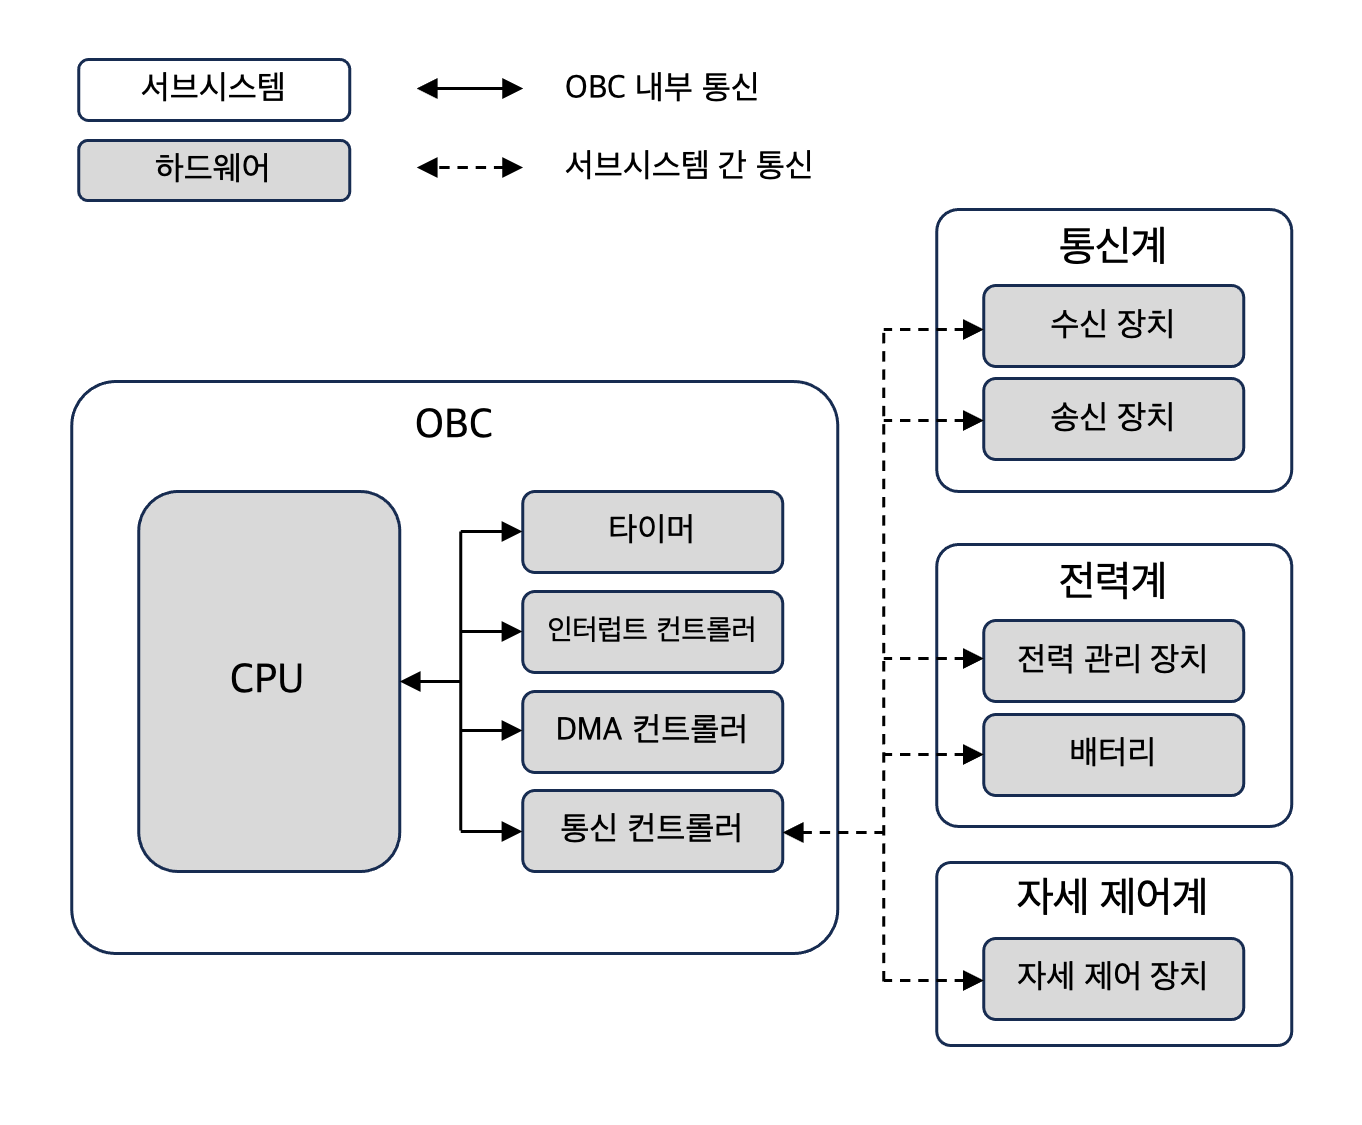
\includegraphics[width=12.5cm]{fig_cubesat_structure}}
    \caption{큐브샛 OBC 중심의 주요 하드웨어 통신 구조 예시
    } \label{fig_cubesat_structure}
\end{figure}

그림 \ref{fig_cubesat_structure}은 큐브샛 OBC를 중심으로 한 주요 하드웨어 통신 구조의 한 예를 나타낸 것이다. OBC 내부에는 CPU와 함께 타이머, 인터럽트 컨트롤러, DMA 컨트롤러, 통신 컨트롤러와 같은 내부 주변장치가 존재할 수 있으며, CPU는 이들을 MMIO 레지스터 접근을 통해 제어한다. 반면 전력계, 배터리, 자세 제어계, RF 송수신 장치 등은 외부 서브시스템에 속한 주변장치로 존재할 수 있으며, OBC는 통신 컨트롤러를 통해 OBC에 노출된 장치와 명령과 응답을 주고받는다. 그림의 실선 화살표는 OBC 내부에서 이루어지는 MMIO 기반 접근을, 점선 화살표는 외부 장치와의 통신 경로를 나타낸다. 이때 외부 서브시스템 사이의 통신 경로는 모든 시스템에서 항상 존재하는 연결을 의미하지 않으며, 임무와 보드 설계에 따라 선택적으로 구성될 수 있는 대표적인 연결 관계를 나타낸다.

이 구조에서 OBC 펌웨어의 실행은 내부 주변장치와 OBC에 노출된 외부 서브시스템 주변장치의 상태에 모두 의존한다. 예를 들어 타이머 카운터 값은 인터럽트 발생 시점을 결정하고, 인터럽트 컨트롤러의 대기 상태는 어떤 핸들러가 실행될지를 결정한다. 또한 OBC에 노출된 외부 주변장치가 반환하는 통신 응답은 명령 처리 결과와 이후 분기 흐름에 영향을 준다. 따라서 펌웨어를 분석할 때에는 명령어 자체의 의미뿐 아니라, 펌웨어가 관찰하는 장치 상태와 통신 결과도 함께 고려해야 한다.

\subsection{통신 흐름}

\begin{figure}[t]
    \centerline{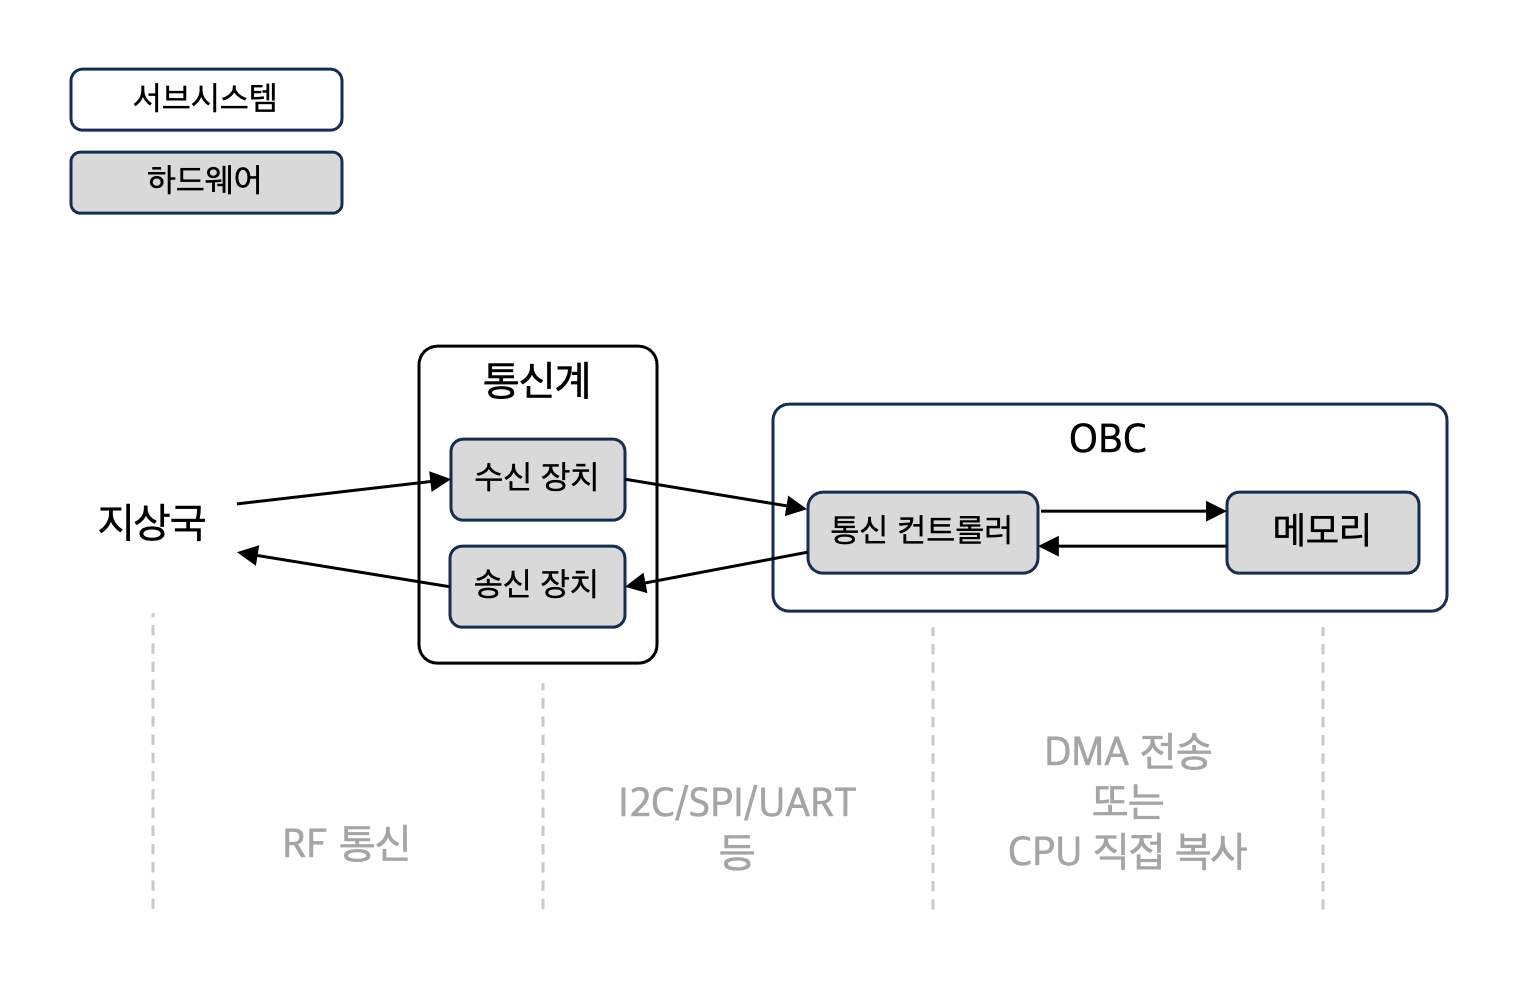
\includegraphics[width=12.5cm]{fig_randev_data}}
    \caption{지상국과 큐브샛 OBC 사이의 명령-응답 통신 흐름 예시
    } \label{fig_cubesat_data_flow}
\end{figure}

큐브샛에서 지상국 명령을 수신하고 그 결과나 위성 상태를 원격 측정 데이터로 송신하는 과정은 OBC 펌웨어만의 역할이 아니라, 펌웨어와 하드웨어 설계가 함께 수행하는 시스템 동작이다. 펌웨어는 통신 인터페이스를 설정하고 메모리에 저장된 패킷을 해석하지만, 실제 RF 송수신, 버퍼링, 버스 전송, 메모리 복사는 주변장치의 상태와 보드 설계에 따라 진행된다. 그림 \ref{fig_cubesat_data_flow}은 지상국과 큐브샛 OBC 사이에서 명령과 응답 데이터가 이동하는 주요 경로를 단순화하여 나타낸 예시이다. 그림의 구성요소와 연결 방식은 일반적인 흐름을 설명하기 위한 것이며, 실제 통신 장치의 명칭, 버스 종류, 버퍼 구성, 데이터 복사 방식은 큐브샛 설계에 따라 달라질 수 있다.

외부에서 전달된 RF 패킷은 통신계의 RF 송수신 장치에 도달한다. OBC는 I2C, SPI, UART와 같은 통신 인터페이스를 통해 이 장치에서 수신 데이터를 읽고, 데이터는 통신 인터페이스의 수신 버퍼 또는 OBC 메모리에 저장된다. 이후 필요한 경우 DMA 전송이나 CPU 복사를 통해 패킷이 펌웨어가 처리할 수 있는 메모리 영역으로 이동한다. 펌웨어는 메모리에 저장된 패킷을 해석하고, 명령 파서와 명령 디스패처를 거쳐 해당 명령 핸들러를 실행한다.

반대 방향의 원격 측정 응답은 OBC 메모리에서 시작된다. 펌웨어가 응답 프레임을 구성하면, 해당 데이터는 CPU 복사나 DMA 전송을 통해 통신 인터페이스의 송신 버퍼로 이동한다. 이후 통신 인터페이스는 응답 데이터를 통신계의 RF 송수신 장치로 전달하고, RF 송수신 장치는 이를 지상국으로 송신한다. 이처럼 명령 수신과 응답 송신은 같은 장치와 버스를 공유할 수도 있고, 설계에 따라 별도의 수신 및 송신 경로로 나뉠 수도 있다.

이러한 통신 흐름은 펌웨어가 단순히 메모리 안의 데이터를 처리하는 프로그램이 아니라, 외부 입력 큐, 통신 장치 응답, 데이터 전송 상태, 송수신 장치의 준비 상태에 따라 실행 경로가 달라지는 시스템 소프트웨어임을 보여준다. 본 연구에서 RF 패킷 큐, 통신 인터페이스의 수신 및 송신 버퍼, 데이터 전송 과정, 외부 주변장치 응답을 모델링하는 이유도 이러한 배경에 있다.

\subsection{작업 및 인터럽트 흐름}

OBC 펌웨어는 외부 명령을 처리하는 동시에 주기적인 상태 점검, 통신 관리, 서브시스템 제어와 같은 여러 작업을 수행한다. 이러한 작업은 단일 루프 안에서 순차적으로 실행될 수도 있지만, 많은 펌웨어에서는 실시간 운영체제 또는 스케줄러를 사용하여 여러 작업 문맥을 전환하며 실행한다. 이때 타이머 인터럽트는 주기적인 스케줄링과 지연 시간 처리를 위한 핵심 입력이 된다.

많은 OBC 펌웨어는 타이머 인터럽트를 기반으로 주기적인 작업 문맥 전환을 수행한다. 타이머 장치는 설정된 클럭과 비교 조건에 따라 인터럽트를 발생시키며, 인터럽트 컨트롤러는 각 인터럽트의 대기 상태와 우선순위를 관리한다. 펌웨어는 인터럽트 핸들러(interrupt handler)에 진입한 뒤 스케줄러 관련 처리를 수행하고, 필요에 따라 현재 작업의 문맥을 저장하거나 다른 작업으로 실행 흐름을 전환한다.

이러한 흐름은 펌웨어 실행에서 인터럽트와 주변장치 상태가 단순한 부가 기능이 아니라 제어 흐름을 결정하는 요소임을 의미한다. 타이머가 동작하지 않으면 주기적인 작업 전환이 일어나지 않고, 인터럽트 컨트롤러가 대기 중인 인터럽트를 관리하지 않으면 핸들러 진입과 문맥 전환이 재현되지 않는다. 따라서 OBC 펌웨어를 실행하거나 실행 기반으로 분석하려면, CPU 명령어 실행뿐 아니라 타이머와 인터럽트 컨트롤러 같은 주변장치의 관찰 가능한 동작도 함께 제공해야 한다.

\section{정적 프로그램 분석}

정적 프로그램 분석은 프로그램을 실제로 실행하지 않고 코드와 데이터의 구조를 분석하는 방법이다. 바이너리 프로그램을 대상으로 하는 정적 분석에서는 기계어 명령어를 역어셈블하고, 함수 경계, 심볼, 데이터 참조, 제어 흐름, 호출 관계를 복원한다. 이러한 정보는 소스 코드가 없거나 제한적으로만 제공되는 펌웨어를 이해하는 데 중요한 단서가 된다.

펌웨어 분석에서 정적 분석은 특히 유용하다. 펌웨어 바이너리만으로도 어떤 함수가 존재하는지, 어떤 주변장치 주소에 접근하는지, 어떤 명령 핸들러가 포함되어 있는지, 어떤 함수들이 서로 호출되는지를 확인할 수 있기 때문이다. 또한 정적 분석 결과는 이후 수동 분석, 취약점 탐색, 테스트 입력 설계, 에뮬레이션 경로 선정의 기반으로 사용될 수 있다.

다만 정적 분석은 프로그램을 실행하지 않기 때문에 실행 시점의 레지스터 값, 메모리 값, 장치 응답, 인터럽트 발생 여부를 직접 관찰하지 못한다. 따라서 실행 중에 결정되는 간접 호출 대상이나 외부 입력에 의해 선택되는 경로는 보수적으로 추정되거나 분석 결과에서 빠질 수 있다. 3장에서는 이러한 특성이 큐브샛 OBC 펌웨어 분석에서 어떤 한계로 나타나는지 구체적으로 설명한다.

\subsection{제어 흐름과 호출 그래프}

정적 분석에서 제어 흐름은 프로그램 실행이 한 명령어 또는 기본 블록에서 다른 명령어 또는 기본 블록으로 이동하는 관계를 의미한다. 함수 내부의 제어 흐름은 보통 제어 흐름 그래프(control-flow graph, CFG)로 표현되며, 조건 분기, 반복문, 직접 분기, 간접 분기와 같은 구조를 포함한다. 함수 사이의 호출 관계는 호출 그래프(call graph)로 표현되며, 어떤 함수가 어떤 함수를 호출할 수 있는지를 보여준다.

직접 호출이나 직접 분기는 명령어 안에 대상 주소가 명시되어 있으므로 비교적 쉽게 복원할 수 있다. 반면 간접 호출과 간접 분기는 대상 주소가 레지스터나 메모리 값으로부터 결정되기 때문에 정적 분석만으로 정확한 대상을 알기 어렵다. 예를 들어 함수 포인터, 분기 테이블, 콜백 구조, 명령 디스패처는 실행 시점의 값에 따라 호출 대상이 결정될 수 있다. 이러한 간접 제어 흐름은 펌웨어의 실제 도달 가능 경로를 이해하는 데 중요하지만, 정적 분석 결과에서는 누락되거나 불완전하게 표현될 수 있다.

본 연구에서 말하는 정적 분석 범위 확장은 주로 이러한 호출 그래프와 도달 가능 함수의 관점에서 다룬다. 실행 중 확인한 간접 제어 흐름 대상을 프로그램 데이터베이스에 반영하면, 기존 정적 분석에서 연결되지 않았던 호출 관계를 추가하고, 그 결과 더 많은 함수가 시작점으로부터 도달 가능한 것으로 분석될 수 있다.

\subsection{프로그램 데이터베이스}

정적 분석 도구는 원본 바이너리와 분석 과정에서 생성한 정보를 내부 저장소에 함께 관리한다. 본 논문에서는 이러한 내부 저장소를 프로그램 데이터베이스라고 부른다. 이는 모든 분석 도구에서 동일하게 사용하는 고정된 용어라기보다, 바이너리와 분석 결과가 함께 저장되는 논리적 저장소를 가리키기 위한 표현이다. 예를 들어 IDA는 분석 결과를 IDB 파일에 저장하고, Ghidra는 프로그램별 데이터베이스에 메모리, 코드, 데이터, 함수, 심볼 등의 정보를 저장한다.

프로그램 데이터베이스에는 단순히 원본 바이너리의 바이트열만 저장되는 것이 아니라, 메모리 블록, 명령어, 데이터 항목, 함수, 심볼, 주석, 참조와 같은 분석 결과가 함께 저장된다. 여기서 참조(reference)는 프로그램 안의 한 위치가 다른 위치를 가리키거나 그 위치로 제어를 이동할 수 있음을 나타내는 정보이다. 호출 그래프와 도달 가능성 분석은 함수와 참조 정보를 바탕으로 구성되므로, 참조가 누락되면 실제로 존재하는 호출 관계가 분석 결과에 반영되지 않을 수 있다. 본 연구에서 실행 중 확인한 간접 제어 흐름을 프로그램 데이터베이스에 반영한다는 것은, 이러한 분석 도구의 내부 저장소에 정적 분석이 재사용할 수 있는 형태로 동적 정보를 추가한다는 의미이다.

\section{Ghidra}

Ghidra는 바이너리 프로그램의 역공학을 지원하는 무료 공개 소프트웨어 분석 프레임워크이다\cite{Ghidra}. Ghidra는 바이너리 가져오기, 역어셈블, 역컴파일, 심볼 및 참조 분석, 함수 생성, 호출 그래프 분석 등 펌웨어 정적 분석에 필요한 기능을 제공한다. 또한 소스 코드가 공개되어 있고 스크립트 및 확장 기능을 제공하므로, 분석 도구 내부의 데이터베이스와 실행 기능을 연구 목적에 맞게 활용하기에 적합하다. 본 연구에서는 Ghidra를 단순한 역어셈블러가 아니라, 펌웨어 실행 결과를 다시 프로그램 데이터베이스에 반영할 수 있는 분석 환경으로 사용한다.

Ghidra를 본 연구의 기반으로 사용한 중요한 이유는 명령어 의미가 P-code라는 아키텍처 독립적인 중간 표현으로 변환되기 때문이다. 이를 활용하면 특정 아키텍처의 명령어 실행기를 새로 구현하지 않고도, Ghidra가 제공하는 P-code 실행 체계 위에서 펌웨어 실행을 관찰할 수 있다. 또한 실행 중 확인된 간접 제어 흐름, 참조, 북마크 등의 정보를 같은 Ghidra 프로그램 데이터베이스에 기록함으로써 기존 정적 분석 결과를 보강할 수 있다.

\subsection{Ghidra 스크립트}

Ghidra 스크립트는 Ghidra 내부의 프로그램 데이터베이스와 분석 기능을 자동화하기 위한 인터페이스이다. 2.3.2절에서 설명한 프로그램 데이터베이스의 개념은 Ghidra에서 프로그램 메모리, 리스팅, 함수, 심볼, 참조(reference), 북마크(bookmark) 등의 객체로 구체화된다. 스크립트를 사용하면 이러한 객체에 접근하고, 필요한 경우 새로운 참조나 북마크와 같은 분석 결과를 데이터베이스에 추가할 수 있다. 또한 Ghidra 스크립트는 그래픽 사용자 인터페이스 환경뿐 아니라 Headless Ghidra 환경에서도 실행될 수 있으므로, 대규모 분석이나 반복 실험을 자동화하는 데 사용할 수 있다.

본 연구의 구현은 Headless Ghidra에서 실행되는 스크립트 형태로 구성된다. 스크립트는 대상 펌웨어를 실행하기 위한 초기 상태를 설정하고, Ghidra의 P-code 실행 기능을 사용하여 명령어를 실행하며, 실행 중 관찰한 MMIO 접근과 간접 제어 흐름을 프로그램 데이터베이스에 기록한다. 따라서 Ghidra 스크립트는 본 연구에서 에뮬레이션, 주변장치 모델 연결, 동적 제어 흐름 기록, 데이터베이스 갱신을 연결하는 실행 환경 역할을 한다.

\subsection{SLEIGH 명세 언어}

SLEIGH는 Ghidra가 프로세서 아키텍처의 명령어 형식과 의미를 정의하기 위해 사용하는 명세 언어이다\cite{SLEIGH}. 각 아키텍처의 SLEIGH 명세는 바이너리 명령어의 비트 패턴, 피연산자 해석 방식, 그리고 해당 명령어가 어떤 P-code 연산으로 변환되는지를 정의한다. 따라서 Ghidra가 특정 명령어 집합 구조(Instruction Set Architecture, ISA)의 SLEIGH 명세를 제공한다면, 분석 도구는 해당 아키텍처의 명령어를 공통된 P-code 표현으로 다룰 수 있다.

예를 들어 AVR32의 \texttt{ICALL}(indirect call) 명령어는 Ghidra의 SLEIGH 명세에서 다음과 같이 정의된다.\footnote{\url{https://github.com/NationalSecurityAgency/ghidra/blob/master/Ghidra/Processors/Atmel/data/languages/avr32a_data_transfer.sinc}}

\begin{verbatim}
# ICALL Format I:
# Operation:  LR <- PC + 2
#             PC <- Rd
# Syntax:     icall Rd
# 0101 1101 0001 dddd

:ICALL rd0 is op4_12=0x5d1 & rd0 {
    tmp:4 = rd0;
    LR = inst_next;
    call [tmp];
}
\end{verbatim}

위 명세에서 앞부분은 \texttt{icall Rd} 명령어의 비트 패턴과 피연산자를 정의하고, 중괄호 내부는 해당 명령어의 의미를 SLEIGH의 P-code 구문으로 표현한다. \texttt{LR = inst\_next}는 다음 명령어 주소를 링크 레지스터에 저장하는 동작을 나타내며, \texttt{call [tmp]}는 \texttt{rd0} 레지스터 값으로 이동하는 간접 호출을 나타낸다. 이처럼 SLEIGH 명세는 아키텍처별 명령어를 Ghidra가 공통적으로 분석하고 실행할 수 있는 중간 표현으로 연결한다.

\subsection{P-code와 PcodeOp}

P-code는 Ghidra의 중간 표현으로, 아키텍처 의존적인 명령어 의미를 일반화된 연산들의 열로 표현한다. 하나의 기계어 명령어는 하나 이상의 PcodeOp으로 변환될 수 있으며, PcodeOp은 P-code를 구성하는 기본 연산 단위이다. 예를 들어 레지스터 복사, 메모리 읽기, 메모리 쓰기, 산술 연산, 조건 분기, 간접 호출은 각각 \texttt{COPY}, \texttt{LOAD}, \texttt{STORE}, 산술 PcodeOp, \texttt{CBRANCH}, \texttt{CALLIND}와 같은 형태로 표현된다.

앞 절의 \texttt{ICALL} 명세는 명령어의 의미를 SLEIGH 구문으로 표현한 것이다. 실제로 RANDEV OBC 펌웨어의 \texttt{service\_dispatcher\_task} 함수에 있는 \texttt{ICALL R0} 명령어를 Ghidra 스크립트로 확인하면 다음과 같은 PcodeOp으로 변환된다.

\begin{verbatim}
address: 8001f4a6
function: service_dispatcher_task
instruction: ICALL R0
pcode:
  (register, 0x1038, 4) COPY (const, 0x8001f4a8, 4)
   ---  CALLIND (register, 0x1000, 4)
\end{verbatim}

위 출력에서 \texttt{COPY}는 다음 명령어 주소를 링크 레지스터에 저장하는 동작에 해당하고, \texttt{CALLIND}는 \texttt{R0}에 저장된 주소로 이동하는 간접 호출에 해당한다. 이는 앞 절의 SLEIGH 명세에서 \texttt{LR = inst\_next}와 \texttt{call [tmp]}로 표현된 동작과 같은 의미이다.

P-code를 사용하면 서로 다른 아키텍처의 명령어도 공통된 실행 단위로 관찰할 수 있다. 본 연구는 이러한 특성을 이용하여 PcodeOp 단위에서 메모리 접근과 제어 흐름을 확인한다. 구체적으로 \texttt{LOAD}와 \texttt{STORE}를 관찰하여 MMIO 접근을 장치 모델과 연결하고, \texttt{CALLIND}, \texttt{BRANCHIND}, \texttt{RETURN}과 같은 제어 흐름 PcodeOp을 관찰하여 실행 중 확인된 간접 제어 흐름 대상을 Ghidra 프로그램 데이터베이스에 반영한다.

\chapter{연구 동기}

본 장에서는 큐브샛 OBC 펌웨어를 정적 분석만으로 분석할 때 발생하는 한계를 설명한다. 2장에서 설명한 것처럼 OBC 펌웨어는 주변장치와 지속적으로 상호작용하면서 실행된다. 이러한 특성은 펌웨어의 실제 제어 흐름을 이해하는 과정에서 정적 분석만으로는 충분하지 않은 지점을 만든다.

\section{OBC 펌웨어 정적 분석의 필요성}

큐브샛 OBC 펌웨어는 위성의 명령 처리, 원격 측정 수집, 통신 관리, 서브시스템 제어와 같은 핵심 기능을 담당한다. 발사 이후에는 펌웨어를 수정하거나 실제 동작을 관찰할 수 있는 기회가 제한되므로, 발사 이전 또는 분석 가능한 시점에 펌웨어의 구조와 실행 경로를 가능한 한 넓게 파악하는 것이 중요하다. 특히 OBC 펌웨어의 결함은 단일 기능 오류에 머무르지 않고, 통신 두절이나 전력 관리 실패와 같이 임무 전체에 영향을 주는 문제로 이어질 수 있다.

그러나 큐브샛 개발 환경에서는 항상 완전한 소스 코드, 실제 하드웨어, 반복 가능한 통합 시험 환경이 제공되는 것은 아니다. 개발 단계가 지났거나 외부에서 확보한 펌웨어를 분석해야 하는 경우에는 바이너리만 사용할 수 있으며, 실제 보드에 접근하더라도 반복 실험을 충분히 수행하기 어려울 수 있다. 이때 Ghidra와 같은 역공학 도구를 이용한 정적 분석은 펌웨어의 구조를 이해하기 위한 현실적인 출발점이 된다.

정적 분석을 통해 분석자는 펌웨어에 포함된 함수, 명령 핸들러, 주변장치 접근 위치, 함수 간 호출 관계를 확인할 수 있다. 예를 들어 특정 MMIO 주소에 접근하는 명령어를 찾으면 펌웨어가 어떤 주변장치를 제어하는지 추정할 수 있고, 호출 그래프를 구성하면 초기화 루틴, 통신 처리 루틴, 작업 스케줄러, 장치별 명령 처리 함수가 어떤 관계로 연결되는지 파악할 수 있다. 이러한 정보는 펌웨어의 동작 이해뿐 아니라, 추가 검증이 필요한 코드 영역을 정하는 데에도 사용된다.

따라서 본 연구는 정적 분석을 대체하려는 것이 아니라, 정적 분석이 제공하는 프로그램 구조와 데이터베이스를 기반으로 삼는다. 문제는 큐브샛 OBC 펌웨어의 많은 실행 경로가 주변장치 상태와 외부 입력에 의해 결정되기 때문에, 정적 분석만으로는 실제 실행 중 형성되는 모든 제어 흐름을 확인하기 어렵다는 데 있다.

\section{정적 분석 기반 접근의 한계}

정적 분석은 프로그램을 실행하지 않고 가능한 제어 흐름을 복원하기 때문에, 실행 시점에 결정되는 값에 의존하는 경로를 정확히 파악하기 어렵다. 일반적인 응용 프로그램에서도 함수 포인터, 콜백, 분기 테이블과 같은 구조는 정적 분석의 난점이 된다. 큐브샛 OBC 펌웨어에서는 여기에 주변장치 레지스터, 인터럽트, DMA 전송 상태, I2C 장치 응답, 무선 패킷 큐와 같은 외부 실행 환경이 추가된다.

예를 들어 펌웨어가 MMIO 레지스터에서 읽은 값을 조건문에 사용한다면, 해당 분기 결과는 장치 상태에 의해 결정된다. 타이머 인터럽트가 발생해야 특정 작업이 실행되는 경우에는 타이머와 인터럽트 컨트롤러가 동작하지 않으면 해당 경로가 나타나지 않는다. 또한 지상국 명령 패킷이 VRX를 통해 들어오고, 펌웨어가 이를 해석하여 명령 핸들러를 호출하는 구조에서는 외부 입력과 I2C 통신 결과가 호출 그래프의 실제 간선을 결정할 수 있다.

이러한 흐름은 정적 분석 결과에서 두 가지 형태의 한계로 나타난다. 첫째, 실행 중에만 결정되는 간접 제어 흐름의 대상이 누락될 수 있다. 함수 포인터나 디스패처를 통해 호출되는 명령 처리 함수는 실제 실행에서는 특정 대상이 선택되지만, 정적 분석 단계에서는 그 대상을 확인하지 못할 수 있다. 둘째, 실행 환경이 없으면 해당 제어 흐름이 관찰되더라도 분석 도구의 프로그램 데이터베이스에 자동으로 반영되지 않는다. 즉 실행 중 대상 주소를 알 수 있는 경우에도, 이를 참조나 호출 그래프 간선으로 저장하지 않으면 이후 정적 분석 과정에서 재사용하기 어렵다.

따라서 큐브샛 OBC 펌웨어 분석에는 두 가지 보완이 필요하다. 하나는 펌웨어가 실행 중 관찰하는 주변장치 상태와 외부 입력을 제공하여 실제 실행 경로를 일부 재현하는 것이고, 다른 하나는 실행 중 확인한 동적 제어 흐름을 분석 도구의 프로그램 데이터베이스에 반영하는 것이다. 본 연구는 이 두 요구를 Ghidra P-code 기반 에뮬레이션과 데이터베이스 보강으로 연결한다.

\subsection{한계 사례}

본 연구의 대상인 RANDEV OBC 펌웨어에서도 이러한 한계가 여러 곳에서 나타난다. RANDEV OBC 펌웨어는 FreeRTOS 기반 작업, 타이머 인터럽트, PDCA/TWIM 기반 I2C 통신, RF 송수신 장치와의 명령-응답 흐름을 함께 사용한다. 이때 기본적인 정적 분석이나 명령어 실행만으로는 다음과 같은 요소를 충분히 재현하기 어렵다.

\begin{itemize}
    \item MMIO 레지스터 접근 시 주변장치의 상태 변화나 인터럽트 플래그 설정과 같은 부수 효과가 발생하지 않는다. 따라서 펌웨어가 장치 상태 레지스터를 읽어 분기하는 경로가 실제와 다르게 진행될 수 있다.
    \item TC의 카운터 값이 증가하지 않으면 틱 인터럽트가 발생하지 않고, INTC가 대기 중인 인터럽트와 우선순위를 관리하지 않으면 인터럽트 핸들러 진입 및 작업 문맥 전환이 재현되지 않는다.
    \item PDCA와 TWIM의 상태가 모델링되지 않으면 메모리와 I2C 장치 사이의 데이터 전송이 진행되지 않는다. 이 경우 펌웨어가 외부 장치 응답을 읽어 명령 처리 경로를 선택하는 흐름을 관찰하기 어렵다.
    \item VRX와 UTX에 해당하는 무선 패킷 큐가 존재하지 않으면 지상국 명령 입력과 원격 측정 응답 송신 흐름을 재현할 수 없다. 따라서 명령 디스패처와 장치별 명령 핸들러가 실제로 호출되는 경로가 호출 그래프에 반영되지 않을 수 있다.
    \item 간접 호출이나 간접 분기의 대상이 실행 중 확인되더라도, 이를 Ghidra 참조와 북마크로 기록하지 않으면 기존 정적 분석 데이터베이스와 연결되지 않는다.
\end{itemize}

대표적인 예로 RANDEV OBC 펌웨어의 인터럽트 진입 루틴에서는 인터럽트 컨트롤러(INTC)의 상태에 따라 실제 핸들러가 동적으로 선택된다. 다음은 \texttt{\_int0} 루틴의 핵심 역어셈블 결과이다.

\begin{verbatim}
_int0_normal:
    MOV        R12, 0x0
    MCALL      PC[->_get_interrupt_handler]
    CP.W       R12, 0x0
    MOV{NE}    PC, R12
    RETE
\end{verbatim}

이 루틴은 먼저 \texttt{\_get\_interrupt\_handler(0)}를 호출하여 핸들러 주소를 \texttt{R12}에 저장한 뒤, 조건부 \texttt{MOV PC,R12} 명령어로 \texttt{R12}가 가리키는 주소로 제어를 이전한다. 이 명령어의 대상은 명령어 안에 직접 인코딩된 고정 주소가 아니라 런타임에 계산된 레지스터 값이므로, 일반적인 정적 호출 그래프에서는 \texttt{\_int0}에서 실제 인터럽트 핸들러로 이어지는 간선이 누락될 수 있다.

이 간접 제어 흐름은 단순한 함수 포인터 호출만의 문제가 아니라 주변장치 상태와도 직접 연결된다. \texttt{\_get\_interrupt\_handler}의 Ghidra 디컴파일 결과는 다음과 같다.

\begin{verbatim}
__int_handler _get_interrupt_handler(uint32_t int_level)
{
  int iVar1;
  int iVar2;

  iVar1 = *(int *)((0x83 - int_level) * 4 + -0x10000);
  iVar2 = *(int *)((iVar1 + 0x40) * 4 + -0x10000);
  if (iVar2 == 0) {
    return (__int_handler)0x0;
  }
  return _int_handler_table[iVar1]
         ._int_line_handler_table[0x1f - LZCOUNT(iVar2)];
}
\end{verbatim}

위 코드에서 \texttt{-0x10000}을 기준으로 한 접근은 32비트 주소 공간의 \texttt{0xffff0000} 영역에 해당하며, 이는 RANDEV OBC에서 INTC 레지스터가 배치된 MMIO 영역이다. \texttt{\_get\_interrupt\_handler}는 INTC 레지스터에서 autovector 값과 대기 중인 인터럽트 비트를 읽고, 그 값을 이용해 \texttt{\_int\_handler\_table}을 인덱싱하여 실제 핸들러 주소를 반환한다. 따라서 \texttt{\_int0}에서 어느 핸들러로 이동하는지는 펌웨어 코드에 고정된 상수만으로 결정되지 않고, 인터럽트 컨트롤러의 런타임 상태와 핸들러 테이블 조회 결과에 의해 결정된다.

이 경우 주변장치 상태가 모델링되지 않으면 \texttt{\_get\_interrupt\_handler}가 읽는 autovector 및 pending bit 값을 알 수 없고, 결과적으로 조건부 \texttt{MOV PC,R12}의 실제 분기 대상도 확인하기 어렵다. 즉 정적 분석 결과에는 \texttt{\_int0}에서 \texttt{\_get\_interrupt\_handler}로의 직접 호출만 나타나고, 실제 인터럽트 핸들러로 이어지는 간접 제어 흐름은 호출 그래프에 반영되지 않을 수 있다. 본 연구에서 에뮬레이션 중 관찰한 간접 제어 흐름 대상을 Ghidra 참조와 북마크로 기록하는 이유는 이러한 누락 간선을 이후 정적 분석에서 재사용할 수 있도록 하기 위함이다.

Ghidra는 프로그램 분석을 위한 에뮬레이션 기능을 제공하지만, 기본 에뮬레이터만으로 이러한 펌웨어 실행 환경이 자동으로 구성되는 것은 아니다. 기본 에뮬레이터는 명령어 의미를 실행할 수 있으나, 특정 MMIO 주소에 대한 읽기와 쓰기가 어떤 장치 동작으로 이어지는지 알지 못한다. 또한 장치 모델이 없으면 타이머, 인터럽트, DMA, I2C, RF 패킷 큐와 같은 상태가 갱신되지 않는다.

이 문제는 단순히 펌웨어가 끝까지 실행되는지의 문제가 아니라, 정적 분석 결과의 완성도와도 연결된다. 주변장치 상태가 주어져야 통과하는 분기, 외부 명령이 들어와야 호출되는 명령 핸들러, 실행 중 레지스터 값으로 결정되는 간접 호출 대상은 모두 호출 그래프와 도달 가능 함수 분석에 영향을 준다. 따라서 본 연구에서는 펌웨어가 관찰하는 실행 환경을 모델링하고, 그 실행 중 확인된 간접 제어 흐름을 Ghidra 프로그램 데이터베이스에 반영하는 접근을 취한다. 다음 장에서는 이를 위한 전체 설계를 설명한다.

\chapter{접근 방법 및 설계}

\section{접근 방법: 에뮬레이션을 통한 프로그램 데이터베이스 보강}

본 연구의 목표는 큐브샛 OBC 펌웨어를 단순히 실행하는 데 그치지 않고, 실행 중 확인한 정보를 정적 분석 도구의 프로그램 데이터베이스에 반영하는 것이다. 3장에서 설명한 것처럼 OBC 펌웨어의 제어 흐름은 MMIO 레지스터 상태, 타이머와 인터럽트, DMA/I2C 전송, 외부 명령 패킷과 같은 실행 환경에 의존한다. 따라서 정적 분석만으로는 실제 실행 중 선택되는 간접 호출 대상이나 명령 처리 경로를 충분히 확인하기 어렵다.

이를 보완하기 위해 본 연구는 정적 분석 도구에 적재된 펌웨어 바이너리를 실행하고, 그 과정에서 관찰한 동적 제어 흐름을 다시 같은 프로그램 데이터베이스에 기록하는 방식을 사용한다. 에뮬레이션은 펌웨어가 주변장치와 상호작용할 수 있는 실행 환경을 제공하고, 데이터베이스 보강은 실행 중 확인된 흐름이 이후의 호출 그래프 및 도달 가능성 분석에서 재사용되도록 한다. 즉 본 연구의 접근은 실행 기반 분석과 정적 분석을 별도의 결과물로 분리하지 않고, 프로그램 데이터베이스를 중심으로 결합하는 데 있다.

이 접근에는 세 가지 기능이 필요하다. 첫째, 펌웨어를 실행하고 실행 중 제어 흐름을 관찰할 수 있는 에뮬레이션 모듈이 필요하다. 둘째, 펌웨어가 MMIO, 인터럽트, I2C 장치 응답과 같은 외부 상태를 관찰할 수 있도록 주변장치 모델을 연결해야 한다. 셋째, 실행 중 확인한 간접 제어 흐름을 별도의 로그로만 남기지 않고 프로그램 데이터베이스에 반영하여 기존 정적 분석 절차가 재사용할 수 있게 해야 한다. 본 연구에서는 이 일반 구조를 Ghidra의 P-code 실행 체계와 프로그램 데이터베이스를 사용하여 구체화한다.

다만 본 연구의 목적은 전체 하드웨어를 주기 정확하게 시뮬레이션하는 데 있지 않다. 본 연구에서 필요한 것은 실제 하드웨어의 모든 내부 상태가 아니라, 펌웨어 실행과 정적 분석 보강에 영향을 주는 관찰 가능한 동작이다. 따라서 장치 모델은 전기적 신호나 센서 물리 모델보다, 펌웨어가 읽는 레지스터 값, 인터럽트 발생 여부, DMA 전송 결과, 통신 응답 바이트, RF 패킷 큐와 같은 요소를 우선한다.

\section{설계 개요}

본 연구의 전체 구조는 그림~\ref{fig_framework}와 같다. 그림은 정적 분석 결과를 실행 중 관찰한 동적 정보로 보강하는 구조를 일반화하여 나타낸 것이다. 펌웨어 바이너리는 먼저 정적 분석기에 의해 분석되고, 그 결과는 펌웨어 데이터베이스에 저장된다. 여기서 펌웨어 데이터베이스는 2.3.2절에서 설명한 프로그램 데이터베이스, 즉 바이너리와 분석 결과를 함께 관리하는 저장소를 의미한다. 큐브샛 에뮬레이터는 같은 펌웨어를 실행하면서 동적 제어 흐름 로그를 생성하고, 데이터베이스 보강 모듈은 기존 펌웨어 데이터베이스와 동적 제어 흐름 로그를 결합하여 보강된 펌웨어 데이터베이스를 만든다.

\begin{figure}[t]
    \centerline{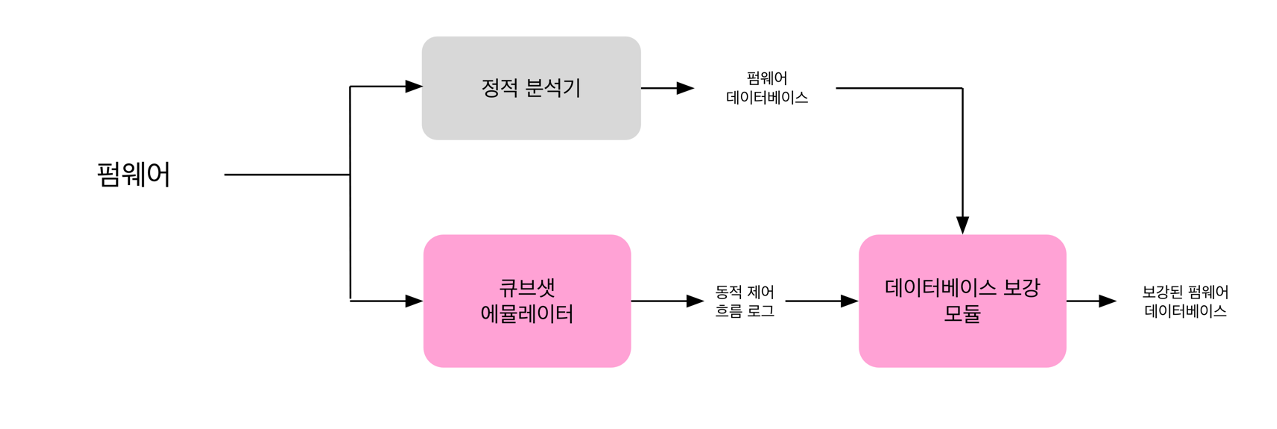
\includegraphics[width=13.5cm]{fig_framework}}
    \caption{에뮬레이션 기반 프로그램 데이터베이스 보강 구조
    } \label{fig_framework}
\end{figure}

본 연구에서는 그림의 일반 구조를 Ghidra 기반으로 구체화하였다. Ghidra는 정적 분석 결과를 프로그램 데이터베이스로 관리하고, 스크립트를 통해 참조와 북마크 같은 분석 정보를 추가할 수 있으며, SLEIGH와 P-code 기반의 실행 체계를 제공한다. 따라서 본 구현에서는 정적 분석기, 프로그램 데이터베이스, 에뮬레이션 모듈, 데이터베이스 보강 모듈을 모두 Ghidra 환경 위에서 연결한다.

구체화된 구조는 P-code 실행 계층, 주변장치 모델 계층, 데이터베이스 보강 계층으로 나눌 수 있다. P-code 실행 계층은 펌웨어 명령어를 실행하고 PcodeOp 단위의 관찰 지점을 제공한다. 주변장치 모델 계층은 실행 중 확인한 메모리 접근과 외부 통신을 펌웨어가 기대하는 장치 동작으로 연결한다. 데이터베이스 보강 계층은 에뮬레이션 중 확인한 동적 제어 흐름을 기존 Ghidra 프로그램 데이터베이스에 반영한다.

\noindent\textbf{P-code 실행 계층.}
본 연구는 새로운 중앙 처리 장치 에뮬레이터를 직접 구현하지 않고, Ghidra의 SLEIGH 명세와 P-code 실행 체계를 재사용한다. 명령어 해석과 의미 변환은 Ghidra가 담당하고, 본 연구의 에뮬레이터는 PcodeOp 단위에서 메모리 접근, 제어 흐름 변화, 사용자 연산이 나타나는 지점을 관찰한다. 이 계층은 특정 명령어 집합을 직접 구현하지 않으면서도, 실행 중 주변장치 모델과 데이터베이스 보강 계층을 호출할 수 있는 공통 관찰 지점을 제공한다.

\noindent\textbf{주변장치 모델 계층.}
주변장치 모델 계층은 펌웨어가 관찰하는 하드웨어 동작을 제공한다. MMIO 주소에 대한 읽기와 쓰기는 일반 메모리 접근과 달리 장치 상태 변화, 인터럽트 발생, 데이터 전송 시작과 같은 부수 효과를 만들 수 있으므로, 실행 중 장치 모델로 전달되어야 한다. 또한 외부 서브시스템에 속한 장치는 통신 인터페이스를 통해 명령과 응답을 주고받는 대상으로 모델링한다. 이 계층에서 중요한 기준은 실제 하드웨어의 모든 내부 동작이 아니라, 펌웨어의 분기와 제어 흐름에 영향을 주는 관찰 가능한 상태이다.

\noindent\textbf{데이터베이스 보강 계층.}
데이터베이스 보강 계층은 에뮬레이션 결과를 외부 로그로만 남기지 않고 Ghidra 프로그램 데이터베이스에 반영한다. 정적 분석만으로 대상이 불명확한 간접 호출이나 간접 분기가 실행 중 특정 주소로 이동한 경우, 그 정보를 참조와 보조 표식 형태로 저장한다. 이렇게 반영된 정보는 이후 호출 그래프 생성과 도달 가능성 분석에서 기존 정적 분석 결과와 함께 사용될 수 있다.

\noindent\textbf{공통 구조와 대상 의존 요소의 분리.}
Ghidra 기반 구체화 안에서도 재사용 가능한 부분과 대상 펌웨어에 의존하는 부분은 구분된다. P-code 실행, PcodeOp 후킹, MMIO 접근 전달, 통신 장치 추상화, 동적 제어 흐름의 데이터베이스 반영 방식은 공통 구조로 둘 수 있다. 반면 실제 펌웨어를 실행하려면 MMIO 기준 주소와 레지스터 의미, 인터럽트 맵, DMA 및 통신 컨트롤러의 전송 규칙, 외부 장치의 명령-응답 규약, 사용자 연산의 의미와 같은 대상별 정보가 필요하다. 이 구분은 본 연구가 모든 큐브샛 펌웨어를 수정 없이 실행하는 완전한 범용 에뮬레이터가 아니라, 정적 분석 데이터베이스를 실행 정보로 보강하는 일반 구조를 Ghidra P-code 실행과 프로그램 데이터베이스로 구체화한 것임을 명확히 한다.

\chapter{구현}

\section{개요}

본 장에서는 4장에서 설명한 접근 방법을 실제 구현으로 구체화한 내용을 설명한다. 구현은 펌웨어 바이너리를 입력으로 받아 OBC의 명령어 실행 계층, 주변장치 모델 계층, 프로그램 데이터베이스 보강 계층을 함께 구성한다. 이때 에뮬레이션 엔진의 구체적인 선택과 실행 방식은 5.2절에서 설명하고, 공통 실행 구조와 구분되는 대상 펌웨어 의존 요소는 5.4절에서 별도로 정리한다.

현재 구현은 이후 실험에서 사용하는 RANDEV OBC 펌웨어를 기준으로 개발되었다. 따라서 코드 수준의 장치 명칭과 일부 세부 메커니즘은 RANDEV 보드와 펌웨어가 사용하는 주변장치 구성을 따른다. 그러나 구현을 구성하는 계층 중 P-code 실행 루프, MMIO 접근 전달, 장치 모델 연결 방식, I2C 명령-응답 추상화, 동적 제어 흐름 기록 및 데이터베이스 반영 방식은 RANDEV에만 닫힌 요소가 아니라 다른 큐브샛 OBC 펌웨어에도 재사용 가능한 공통 구조로 볼 수 있다. 본 장에서는 이 점을 염두에 두고 RANDEV 기준으로 구현된 요소 중 재사용 가능한 기능 범주와 대상별로 교체해야 하는 정보를 구분하여 설명한다.

구현은 크게 세 부분으로 구성된다. 첫째, OBC CPU의 명령어 실행을 소프트웨어로 대체하여 펌웨어를 실행하는 OBC 펌웨어 에뮬레이터이다. 둘째, MMIO 장치와 통신 기반 외부 장치 모델을 연결하여 펌웨어가 기대하는 주변장치 동작을 제공하는 장치 모델 계층이다. 셋째, 실행 중 관찰한 간접 제어 흐름을 정적 분석 데이터베이스에 기록하는 프로그램 데이터베이스 보강 계층이다.

\section{OBC 펌웨어 에뮬레이터}

2장에서 살펴본 큐브샛 구조에서 OBC 펌웨어의 실행은 CPU, 내부 주변장치, OBC에 노출된 외부 서브시스템 주변장치가 함께 동작하는 과정으로 나타난다. 따라서 OBC 펌웨어를 소프트웨어만으로 실행하려면 그림~\ref{fig_cubesat_structure}의 구성요소를 하나씩 소프트웨어 구성요소로 대체해야 한다. CPU는 펌웨어 명령어를 실행하는 에뮬레이션 엔진으로, MMIO로 접근되는 내부 주변장치는 레지스터와 부수 효과를 가진 장치 모델로, OBC에 노출된 외부 서브시스템 주변장치는 통신 인터페이스를 통해 명령과 응답을 주고받는 장치 모델로 대응된다. 그림~\ref{fig_cubesat_structure}은 이러한 기능 범주를 일반화하여 나타낸 것이며, 표~\ref{tab:randev-device-model}은 같은 구조가 현재 구현에서 어떤 RANDEV 기준 장치 모델로 구체화되었는지를 정리한 것이다.

본 구현의 목표는 실제 하드웨어의 전기적 동작이나 주기 정확성을 모두 재현하는 것이 아니라, 펌웨어가 실행 중 관찰하는 상태와 이벤트를 제공하는 것이다. 이를 위해 명령어 실행, MMIO 접근, 인터럽트, DMA 전송, I2C 명령-응답 흐름을 소프트웨어적으로 연결하였다. 이러한 구성요소는 RANDEV에만 특수한 기능이라기보다, 주기적인 작업 수행, 전력 및 자세 제어, 원격 명령 수신과 원격 측정 송신이 필요한 대부분의 큐브샛 및 인공위성 OBC에서 반복적으로 나타나는 기능이다.

본 절에서 설명하는 주변장치 모델은 RANDEV OBC 펌웨어를 실행하기 위해 먼저 설계 및 구현되었다. 따라서 TC, INTC, PDCA, TWIM, EPS, ADCS, VRX, UTX와 같은 장치 명칭과 세부 레지스터 동작은 RANDEV 실행 환경을 기준으로 한다. 그러나 이 장치들이 담당하는 역할은 특정 위성에만 닫힌 동작이라기보다, 큐브샛 OBC에서 반복적으로 등장하는 기능 범주와 연결 방식에 해당한다. 실제 적용 시에는 대상 보드의 주소 맵, 레지스터 의미, 인터럽트 연결, DMA 채널, I2C 주소, 명령-응답 규약에 맞게 모델을 구체화해야 하며, 대상에 따라 본 구현에 포함되지 않은 주변장치 모델을 추가해야 할 수도 있다. 또한 모든 하드웨어를 같은 상세도로 모델링할 필요는 없다. 분석 목적과 펌웨어 실행 경로에 따라 어떤 장치는 레지스터별 부수 효과까지 구현하고, 어떤 장치는 초기화 루틴이 기대하는 기본 상태값이나 제한적인 응답만 제공하는 추상화 수준으로 둘 수 있다.

\begin{table}[h]
\caption{RANDEV 기준 구현에서 모델링한 주요 주변장치}
\label{tab:randev-device-model}
\begin{center}
\begin{small}
\begin{tabular}{p{2.4cm}p{3.6cm}p{6.4cm}}
\hline\hline
구분 & 본 구현의 대응 장치 & 역할 \\
\hline
타이머 & TC & 주기적인 카운터 증가와 인터럽트 발생을 통해 작업 지연 및 스케줄링 흐름 제공 \\
인터럽트 컨트롤러 & INTC & 주변장치의 인터럽트 요청을 관리하고 우선순위에 따라 핸들러 진입 결정 \\
DMA 컨트롤러 & PDCA & 메모리와 통신 컨트롤러 사이의 데이터 전송을 수행하여 패킷 송수신 경로 재현 \\
통신 컨트롤러 & TWIM & I2C 트랜잭션을 시작하고 외부 서브시스템 장치와 바이트 단위 송수신 수행 \\
외부 서브시스템 장치 & EPS, ADCS, VRX, UTX 등 & 전력 상태, 자세 제어 상태, RF 송수신 등 OBC가 명령과 원격 측정에서 관찰하는 응답 제공 \\
\hline\hline
\end{tabular}
\end{small}
\end{center}
\end{table}

\subsection{에뮬레이션 엔진 선택}

가장 먼저 결정해야 할 요소는 CPU를 대체할 명령어 실행 엔진이다. 이 계층은 펌웨어 바이너리를 입력으로 받아 명령어를 실행하고, 실행 중 발생하는 메모리 접근과 제어 흐름 변화를 주변장치 모델 및 데이터베이스 보강 계층에 전달한다. 따라서 에뮬레이션 엔진은 단순히 펌웨어를 빠르게 실행하는 기능뿐 아니라, 정적 분석 데이터베이스와의 결합 가능성도 함께 고려하여 선택해야 한다.

대표적인 선택지는 QEMU와 같은 외부 시스템 에뮬레이터를 사용하는 것이다. QEMU는 동적 바이너리 변환을 기반으로 게스트 명령어를 호스트에서 실행 가능한 형태로 변환하며, 임베디드 펌웨어 에뮬레이션에서도 널리 사용된다\cite{QEMU}. QEMU를 사용하면 실행 속도와 시스템 에뮬레이션 측면에서 장점을 얻을 수 있고, 대상 보드의 장치 모델을 구현하면 펌웨어가 기대하는 하드웨어 환경도 재현할 수 있다. 그러나 QEMU는 Ghidra와 별도의 실행 환경이므로, 실행 중 관찰한 간접 제어 흐름을 Ghidra 프로그램 데이터베이스에 반영하려면 실행 로그 수집, 주소 및 함수 경계 매핑, 참조와 북마크 추가를 위한 후처리 절차가 필요하다.

다른 선택지는 Ghidra 스크립트에서 Ghidra의 P-code 실행 체계를 직접 사용하는 것이다. Ghidra는 SLEIGH 명세를 통해 여러 프로세서 아키텍처의 명령어를 P-code로 변환하며, 본 연구에서 사용한 Ghidra 배포판에도 AVR32를 포함한 다수의 프로세서 명세가 포함되어 있다\cite{Ghidra,SLEIGH}. 따라서 대상 아키텍처에 대한 SLEIGH 명세가 존재한다면 별도의 CPU 해석기를 새로 작성하지 않고도 P-code 단위 실행을 재사용할 수 있다. 또한 Ghidra 내부에서 실행되므로, 에뮬레이션 중 관찰한 제어 흐름을 같은 프로그램 데이터베이스의 참조와 북마크로 곧바로 기록할 수 있다.

본 연구의 목적은 가장 빠른 펌웨어 실행이 아니라, 실행 중 확인한 정보를 정적 분석 데이터베이스에 결합하여 분석 범위를 확장하는 것이다. 따라서 본 구현에서는 QEMU 대신 Ghidra P-code 기반 에뮬레이션을 선택하였다. 이 선택은 실행 속도 측면에서는 불리할 수 있지만, PcodeOp 단위 후킹, Ghidra 프로그램 데이터베이스 접근, 참조 및 북마크 기록을 하나의 Headless Ghidra 스크립트 안에서 연결할 수 있다는 장점을 가진다.

\subsection{PcodeOp 단위 실행}

앞 절에서 Ghidra P-code 기반 에뮬레이션을 선택하였으므로, 실제 구현에서는 Headless Ghidra 환경에서 대상 프로그램을 대상으로 스크립트를 실행하였다. 이때 중요한 구현 목표는 명령어 하나를 한 번에 실행하는 것이 아니라, 명령어가 변환된 PcodeOp을 하나씩 관찰하면서 MMIO 접근과 사용자 연산을 중간에서 처리할 수 있도록 실행 루프를 구성하는 것이다.

Ghidra는 스크립트 수준에서 비교적 쉽게 에뮬레이션을 수행할 수 있도록 EmulatorHelper를 제공한다. EmulatorHelper는 프로그램 메모리 적재, 초기 레지스터 상태 설정, 메모리 오류 처리 등 에뮬레이션에 필요한 기본 실행 환경을 자동으로 구성해 주는 보조 클래스이다. 그러나 EmulatorHelper가 기본적으로 생성하는 에뮬레이터는 기존 체계의 DefaultEmulator이며, 사용자에게 제공되는 \texttt{run()}과 \texttt{step()} 인터페이스는 명령어 단위 실행을 중심으로 설계되어 있다. 내부적으로는 각 명령어가 P-code로 변환된 뒤 Emulate 클래스의 실행 루프에서 PcodeOp 단위로 처리되지만, 단일 PcodeOp을 실행하는 메서드는 외부에서 직접 호출할 수 없도록 구현되어 있다. 따라서 EmulatorHelper만을 사용할 경우 명령어 실행 도중 개별 PcodeOp을 관찰하거나, 특정 PcodeOp에서 주변장치 모델을 호출하는 방식의 세밀한 후킹을 구현하기 어렵다.

이러한 이유로 본 구현에서는 Ghidra의 PcodeEmulator 계열을 직접 활용하였다. PcodeEmulator 자체는 공개 클래스이며, 여기서 생성되는 PcodeThread는 \texttt{stepInstruction()}뿐 아니라 \texttt{stepPcodeOp()}을 공개 메서드로 제공한다. 따라서 PcodeThread를 사용하면 명령어 단위 실행뿐 아니라 PcodeOp 단위 실행 제어도 가능하다. 다만 PcodeEmulator를 단순히 직접 생성하면 EmulatorHelper가 제공하던 프로그램 메모리 적재, 초기 레지스터 설정, 메모리 오류 처리 등의 초기 실행 환경을 별도로 연결해야 한다.

본 연구에서는 이러한 초기화 과정을 다시 구현하지 않고, EmulatorHelper가 제공하는 EmulatorConfiguration을 재사용하였다. 구체적으로는 EmulatorHelper를 생성한 뒤 이를 인자로 AdaptedEmulator를 구성하고, Java reflection을 사용하여 AdaptedEmulator 내부의 \texttt{newPcodeEmulator(EmulatorConfiguration)} 메서드를 호출하였다. AdaptedEmulator는 기존 Emulator 인터페이스와 PcodeEmulator 구현을 연결하기 위해 Ghidra에서 제공하는 전환용 클래스이다. 외부에는 기존 에뮬레이터 인터페이스처럼 보이지만, 내부적으로는 PcodeEmulator 기반으로 명령어를 실행한다. 또한 내부의 AdaptedPcodeEmulator는 EmulatorHelper가 제공하는 프로그램 메모리 이미지와 메모리 오류 처리 방식을 사용하므로, Ghidra 프로그램에 적재된 펌웨어 상태를 그대로 활용할 수 있다. 따라서 이 경로를 사용하면 Ghidra가 구성한 프로그램 메모리 적재 방식을 유지하면서도, 실행 루프에서는 \texttt{PcodeThread.stepPcodeOp()}을 통해 PcodeOp 단위 후킹을 수행할 수 있다.

\subsection{MMIO 장치 모델링 및 연결}

펌웨어와 주변장치 간의 MMIO 통신은 메모리 접근이 발생하는 PcodeOp에 대한 후킹을 통해 처리하였다. PcodeOp 단위 실행 중 \texttt{LOAD} 또는 \texttt{STORE}가 나타나면 해당 PcodeOp의 대상 메모리 주소를 검사한다. 접근 주소가 MMIO 주소 범위에 속하면 일반 메모리 접근으로 처리하지 않고, 해당 주소가 속한 MMIO 장치와 레지스터를 찾은 뒤 장치 모델의 \texttt{read} 또는 \texttt{write} 동작으로 전달한다.

MMIO 모델은 MmioDevice와 MmioRegion의 계층 구조로 구성되어 있다. 하나의 주변장치는 MmioDevice로 표현되며 MMIO 기준 주소, 주소 범위의 크기, 인터럽트 그룹, 레지스터 테이블을 가진다. 이때 주변장치 내부에 반복되는 하위 구조가 존재하는 경우 이를 하위 MmioRegion으로 분리한다. 예를 들어 PDCA의 레지스터 메모리 맵에는 각 DMA 채널마다 동일한 레지스터 블록(register block)이 존재하는데, 이를 PDCAChannel이라는 MmioRegion으로 분리한 뒤 PDCA 내부에 여러 개의 PDCAChannel을 만드는 식이다. MmioRegion 역시 하위 MmioRegion을 가질 수 있으며, 각 MmioRegion은 최상위 MmioDevice의 레지스터 테이블에 자신의 오프셋을 기준으로 레지스터를 등록한다. 이를 통해 MmioDevice에 대한 메모리 접근이 발생하였을 때, 각 MmioRegion을 하나하나 탐색하지 않고 곧바로 어느 레지스터에 대한 접근인지 결정할 수 있다.

공통 실행 루프는 장치의 구체적인 레지스터 의미를 직접 알지 않고, \texttt{DeviceManager}를 통해 접근 주소에 맞는 장치 모델을 찾는다. 이후 각 장치 모델이 자신의 레지스터 읽기/쓰기, 인터럽트 요청, DMA 전송, I2C 송수신 동작을 처리한다.

\subsection{인터럽트 처리 및 실행 루프 연동}

TC와 INTC는 모두 MMIO로 접근되는 주변장치이므로, 레지스터 읽기와 쓰기 자체는 앞 절에서 설명한 MMIO 장치 모델링 구조를 통해 처리된다. 그러나 인터럽트는 특정 레지스터 값을 갱신하는 것만으로는 충분하지 않다. 인터럽트는 CPU의 실행 흐름을 비동기적으로 바꾸는 사건이므로, 에뮬레이터의 주 실행 루프가 이를 인식하고 핸들러로 제어를 넘길 수 있어야 한다.

예를 들어 TC는 내부 클럭에 따라 주기적으로 카운터 값을 증가시키며, 비교값에 도달하거나 오버플로가 발생하면 인터럽트 플래그를 설정한다. 본 구현에서는 이러한 동작을 TC 모델의 상태 변화로 표현하고, 연결된 INTC에 인터럽트 요청을 전달하도록 하였다. INTC는 인터럽트 그룹과 각 라인별 대기 비트를 관리하며, 우선순위 레지스터 값을 기준으로 현재 처리 가능한 가장 높은 우선순위의 인터럽트 핸들러 오프셋을 저장한다.

이후 주 에뮬레이션 루프에서는 각 명령어 실행 후 현재 처리 가능한 인터럽트가 있는지 확인한다. 이때 INTC에 들어온 인터럽트가 존재하고 해당 인터럽트가 마스크된 상태가 아니라면 인터럽트에 진입한다. 인터럽트 진입은 데이터시트의 내용에 따라 현재 실행 문맥의 주요 레지스터 및 PC, SR을 스택에 저장하고, SR의 모드 비트와 인터럽트 마스크 비트를 갱신한 뒤 EVBA 기반 핸들러 주소를 계산하여 PC를 이동시키는 방식으로 구현하였다.

\subsection{I2C 장치 모델링 및 연결}

실제 하드웨어에서 OBC와 주변장치 간의 I2C 통신은 TWIM 및 PDCA와의 상호작용을 통해 이루어진다. PDCA는 메모리와 TWIM의 THR/RHR(transmit/receive holding register) 간의 DMA 기반 전송을, TWIM은 THR/RHR과 주변장치 간의 실제 통신을 담당한다. 이러한 통신 방식을 에뮬레이터의 TWIM 및 PDCA 모델에도 반영하였다.

펌웨어가 TWIM 레지스터에 명령을 기록하면 TWIM 모델은 슬레이브 주소, 읽기/쓰기 비트, 전송 길이, START/STOP 플래그를 해석하여 I2C 통신을 수행할 수 있는 상태가 된다. I2C 장치에 값을 쓰는 경우 TWIM의 THR(transmit holding register)로 전달된 바이트를 해당 슬레이브 주소의 I2C 장치로 전달하고, 읽어오는 경우 해당 장치에게서 응답을 받아 TWIM의 RHR(receive holding register)에 저장한다.

PDCA의 경우 펌웨어가 PDCA 채널에 대상 주소와 주변장치, 통신 횟수 및 방향 등을 설정하면 각 채널에서 통신을 시작한다. PSR(peripheral select register)은 통신 대상 주변장치를 나타내며, TWIM의 수신/송신 준비 상태를 확인한 뒤 메모리와 TWIM 레지스터 사이의 바이트, 하프워드, 워드 단위 전송을 수행한다.

각 I2C 장치는 I2CDevice 추상 클래스를 상속하여 구현하였다. \texttt{tx} 메서드는 OBC가 장치로 보내는 명령 또는 페이로드 바이트를 처리하고, \texttt{rx}는 장치가 OBC로 반환할 응답 바이트를 제공한다. 또한 START\_SEND, START\_RECV, FINISH, NACK 이벤트를 통해 트랜잭션 시작과 종료 시점의 상태 초기화, 명령 확정, 패킷 큐 갱신 등을 수행한다. 현재 구현에는 EPS, UTX, VRX, HSTX, ADCS, UVANT 등의 장치 모델이 포함되어 I2C 통신을 수행하도록 구현되어 있다.

VRX/UTX 구현 이후에는 EPS, UVANT, ADCS, HSTX 장치 모델을 추가하였다. 각 장치의 응답은 QEMU 에뮬레이터 구현과 RANDEV 소스 코드를 함께 참고하여 구성하였다. ADCS는 내부 로직이 거의 없는 골격(skeleton) 형태였으므로 에뮬레이터에서도 동일하게 골격 형태로 구현하였다. UVANT의 경우 QEMU 구현에서 응답 길이만 지정되고 응답 버퍼가 갱신되지 않는 명령이 있어, 소스 코드와 QEMU 구현을 함께 참조하여 명령별 응답을 별도로 설정하였다.

\section{프로그램 데이터베이스 보강}

\subsection{동적 제어 흐름 로그 구현}

동적 제어 흐름 로그는 에뮬레이션 실행 중 명령어 실행 전후의 프로그램 카운터를 비교하여 생성한다. 실행 루프는 각 명령어의 실행 전 주소와 실행 후 주소를 확인하고, 정적 분석 결과에서 계산된 흐름(computed flow)으로 표시된 명령어가 실제로 어느 주소로 이동했는지 판단한다. 이때 순차 실행(fallthrough)으로 진행된 경우는 동적 제어 흐름 보강 대상에서 제외한다.

기록 대상은 계산된 호출과 계산된 분기이다. 명령어의 흐름 유형이 computed call 또는 computed jump인 경우, 로그에는 출발지 주소, 도착지 주소, 참조 유형, 기록 이유, 외부 대상 허용 여부를 저장한다. 같은 출발지와 도착지, 참조 유형, 기록 이유를 가진 흐름이 여러 번 관찰되면 한 번만 기록하여 반복 실행으로 인한 중복을 줄인다. 이 로그는 실행 중 관찰한 동적 흐름을 데이터베이스 반영 단계로 넘기기 위한 중간 표현이며, 이 단계에서는 아직 Ghidra 프로그램 데이터베이스에 참조나 북마크를 추가하지 않는다.

일반적인 계산된 흐름 외에 userop에 의해 발생하는 흐름도 별도로 기록한다. 일부 AVR32 명령어는 SLEIGH 명세에서 \texttt{CALLOTHER}를 포함하는 형태로 변환되며, 이 경우 일반적인 FlowType만으로는 실행 후 프로그램 카운터 변화를 충분히 포착하지 못할 수 있다. 이를 위해 PcodeOp 실행 중 \texttt{CALLOTHER}가 나타나면 실행 후 프로그램 카운터를 기준으로 userop 흐름을 기록한다. Supervisor call 계열은 계산된 호출로, 그 외 userop 기반 프로그램 카운터 변화는 계산된 분기로 다룬다.

\subsection{데이터베이스에 동적 제어 흐름 반영}

데이터베이스 보강 단계는 앞 절에서 생성한 동적 제어 흐름 로그를 입력으로 수행된다. 에뮬레이션이 종료되면 로그에 저장된 각 항목을 읽어 주소와 참조 유형을 복원하고, 이를 Ghidra 프로그램 데이터베이스의 참조와 북마크로 반영한다. 이렇게 로그 생성 단계와 데이터베이스 반영 단계를 분리하면, 실행 중 관찰한 흐름을 먼저 보존한 뒤 어떤 항목이 실제 분석 데이터베이스에 추가되었는지 확인할 수 있다.

각 로그 항목을 처리할 때에는 먼저 출발지 주소의 명령어와 함수 정보를 확인하고, 도착지 주소가 어떤 함수에 포함되는지 확인한다. 출발지 함수가 없거나 명령어를 찾을 수 없는 경우에는 해당 항목을 반영하지 않는다. 또한 일반적인 계산 흐름에서 도착지 함수가 확인되지 않거나, 도착지가 출발지와 같은 함수 내부에 머무르는 경우에는 호출 그래프 보강에 직접적인 의미가 작으므로 참조 추가 대상에서 제외한다. 새로운 함수 간 흐름으로 판단되면 Ghidra ReferenceManager를 통해 출발지 명령어 주소에서 도착지 주소로 \texttt{COMPUTED\_CALL}, \texttt{CONDITIONAL\_COMPUTED\_CALL}, \texttt{COMPUTED\_JUMP}, \texttt{CONDITIONAL\_COMPUTED\_JUMP} 중 적절한 참조를 추가한다. 이미 동일한 흐름 참조가 존재하는 경우에는 중복으로 추가하지 않는다.

또한 간접 제어 흐름 위치가 에뮬레이션 중 한 번 이상 확인되었음을 표시하기 위해 북마크를 함께 기록한다. 북마크 종류는 \texttt{DynamicFlow}, 범주는 \texttt{IndirectFlowCovered}로 설정하였으며, 주석에는 흐름이 기록된 이유와 대상 주소를 저장한다. 동일한 출발지 명령어에서 여러 대상이 관찰될 경우에는 기존 북마크 주석에 새로운 대상 정보를 추가한다. 이후 호출 그래프 분석 단계에서는 이 북마크를 이용하여 간접 제어 흐름 위치 확인 비율을 계산하고, 참조 정보를 이용하여 새롭게 확인된 간선을 호출 그래프에 반영한다.

데이터베이스 반영은 하나의 Ghidra transaction 안에서 수행되어, 반영 과정이 끝났을 때 추가된 참조와 북마크가 프로그램 데이터베이스에 확정된다. 에뮬레이션 종료 후에는 로그에 기록된 흐름 수, userop 흐름 수, 실제로 추가된 참조 수, 중복 또는 함수 정보 부족으로 제외된 항목 수를 요약하여 남긴다. 이렇게 반영된 데이터베이스는 6장에서 수행한 호출 그래프 도달 가능성 분석 및 간접 제어 흐름 확인 비율 계산의 입력으로 사용된다.

\section{대상 펌웨어 의존 요소}

현재 구현은 RANDEV OBC 펌웨어를 기준으로 개발되었기 때문에, 공통 구현으로 분류할 수 있는 부분에도 RANDEV의 장치 구성과 실행 흐름이 설계의 출발점으로 반영되어 있다. 따라서 본 연구의 구현을 처음부터 대상 정보를 완전히 제거한 범용 에뮬레이터로 볼 수는 없다. 다만 구현 안에는 다른 펌웨어에도 재사용 가능한 구조와 대상별로 교체해야 하는 정보가 함께 존재하므로, 이를 구분하여 정리할 필요가 있다.

공통 실행 루프는 PcodeOp 실행, MMIO 접근 감지, userop 감지, 간접 제어 흐름 기록을 담당한다. 또한 타이머, 인터럽트 컨트롤러, DMA, I2C, RF 송수신 큐와 같은 주변장치 모델은 RANDEV의 명칭과 세부 레지스터 구성을 기준으로 구현되었지만, 여러 OBC 펌웨어에서 반복되는 기능 범주와 연결 방식을 구현한 패턴으로 재사용할 수 있다. 반면 실제 주소 맵, 레지스터 의미, 통신 규약, 일부 실행 보정은 대상별로 제공되어야 한다.

대상 의존 요소 중 첫 번째는 메모리 맵과 장치 구성이다. DeviceManager는 RANDEV OBC에서 사용되는 MMIO 장치의 기준 주소와 I2C 장치 주소를 등록한다. 예를 들어 PDCA, TC, INTC, TWIM은 MMIO 장치로 등록되고, EPS, VRX, UTX, HSTX, ADCS, UVANT는 I2C 장치로 등록된다. 새로운 펌웨어에 적용하려면 이 장치 목록, 기준 주소, 인터럽트 그룹, I2C 슬레이브 주소를 대상 보드에 맞게 바꾸어야 한다. 또한 대상 보드가 본 구현에 포함되지 않은 버스, 센서, 저장장치, 통신 장치에 의존한다면 해당 주변장치 모델을 추가로 구현해야 한다.

두 번째는 장치별 레지스터 의미와 부수 효과이다. 같은 MMIO 접근이라도 어떤 레지스터에 쓰였는지에 따라 타이머 시작, 인터럽트 플래그 설정, DMA 전송 요청, I2C 트랜잭션 시작과 같은 서로 다른 동작이 발생한다. 본 구현에서는 이러한 동작을 각 장치 클래스의 읽기/쓰기 메서드에 배치하였다. 따라서 공통 실행 루프는 주소 접근을 장치 모델로 전달하기만 하고, 실제 부수 효과는 대상 장치 모델이 결정한다. 다만 모든 장치를 동일한 수준으로 상세하게 구현할 필요는 없다. 펌웨어가 특정 레지스터 값을 읽거나 초기화 성공 여부만 확인하는 경우에는 제한적인 상태값만 반환하는 추상 모델로 충분할 수 있고, 실행 경로와 제어 흐름에 직접 영향을 주는 장치는 인터럽트, DMA, 버퍼 상태와 같은 부수 효과를 더 자세히 구현해야 한다.

세 번째는 외부 장치의 명령-응답 규약이다. VRX와 UTX는 RF 패킷 큐를 통해 외부 명령 입력과 원격 측정 송신을 재현하며, EPS, HSTX, ADCS, UVANT 등은 I2C 명령에 대한 응답 페이로드를 제공한다. 이러한 응답은 펌웨어가 명령 처리 경로를 진행하기 위해 관찰하는 값이므로, 대상 펌웨어와 장치 규약에 맞게 정의되어야 한다.

네 번째는 아키텍처 및 펌웨어별 보정이다. AVR32 SLEIGH 명세에서 userop으로 남는 SCALL, RETE, RETS, SLEEP 등은 별도의 userop 구현이 필요하다. 또한 RANDEV 펌웨어의 FreeRTOS 작업 상태를 추적하기 위해 TCB 주소와 필드 오프셋을 사용한 작업 모니터링도 포함하였다. 이러한 요소는 P-code 실행 구조 자체에는 포함되지 않는 대상 의존 구현이며, 다른 펌웨어에 적용할 때에는 해당 펌웨어의 ISA, RTOS, 보드 구조에 맞게 수정되어야 한다.

이처럼 본 구현의 일반성은 모든 대상별 정보를 제거했다는 의미가 아니라, RANDEV 기준으로 구체화된 구현 안에서 재사용 가능한 실행, 연결, 기록 구조와 대상별 조정이 필요한 정보를 구분할 수 있다는 데 있다. 6장에서는 이 구조를 RANDEV OBC 펌웨어에 적용하기 위해 수행한 주변장치 모델 구체화, 초기 실행 상태 보정, 실험 구성을 설명한다.

\chapter{실험 및 결과}

이 장에서는 제안한 큐브샛 펌웨어 에뮬레이터가 RANDEV OBC 펌웨어를 실제로 실행할 수 있는지, 그리고 실행 과정에서 관찰한 동적 정보를 Ghidra 프로그램 데이터베이스에 반영하여 정적 분석 범위를 확장할 수 있는지를 평가한다. 평가를 위해 다음 세 가지 연구 질문을 설정하였다.

\begin{itemize}
    \item 연구 질문 1: 제안한 에뮬레이터는 원격 측정 명령에 대해 기대한 응답을 반환하는가?
    \item 연구 질문 2: 제안한 에뮬레이터는 프로그램 데이터베이스를 보강할 수 있는가?
    \item 연구 질문 3: 보강된 데이터베이스로 정적 분석을 시행했을 때 기존보다 더 넓은 범위를 분석할 수 있는가?
\end{itemize}

모든 실험은 8 vCPU와 32GB RAM이 장착된 Ubuntu 22.04 장비에서 진행하였으며, 에뮬레이터는 Headless Ghidra 환경에서 Ghidra 스크립트 형태로 실행하였다.

\section{실험 대상: RANDEV OBC 펌웨어}

실험은 Ghidra에 가져온 RANDEV OBC 펌웨어 바이너리를 대상으로 수행하였다. 평가 대상 펌웨어는 AVR32 기반 환경에서 동작하며, MMIO를 통해 내부 주변장치를 제어하고 I2C를 통해 EPS, ADCS, VRX, UTX, HSTX 등 외부 장치와 통신한다. 본 연구에서 RANDEV를 대상으로 선택한 이유는 타이머, 인터럽트, DMA, I2C, RF 송수신 흐름 등 큐브샛 OBC 펌웨어 실행에 필요한 주요 요소가 함께 나타나며, 기존 QEMU 실행 결과와 일부 소스 코드를 참조하여 에뮬레이터 동작을 검증할 수 있기 때문이다.

RANDEV 개발자로부터 제공받은 펌웨어 소스 코드는 장치 모델의 응답 형식, 통신 순서, 기존 실행 결과를 확인하기 위한 보조 자료로 사용하였다. 그러나 에뮬레이션과 데이터베이스 보강의 직접 대상은 소스 코드가 아니라 Ghidra 프로그램 데이터베이스에 적재된 펌웨어 바이너리이다.

펌웨어 실행 및 원격 측정 응답 검증에는 6.2.4절에서 설명하는 TCP 클라이언트를 사용하였다. TCP 클라이언트는 원격 측정 패킷을 전송하고, 펌웨어가 UTX를 통해 생성한 응답을 다시 수신한다. 전송 대상은 RANDEV 펌웨어가 외부 명령 핸들러 수준에서 처리하는 I2C 장치 명령으로 제한하였다. 이는 I2C 장치 모델 자체에는 존재하더라도 펌웨어 단계에서 외부 원격 측정 명령으로 노출되지 않는 명령을 실험 대상에서 제외하기 위한 기준이다.

본 연구가 목표로 하는 것은 주기 정확 하드웨어 시뮬레이션이 아니다. 대신 펌웨어가 실행 중 관찰하는 레지스터 값, 인터럽트, 패킷, 명령 응답과 같은 관찰 가능한 동작을 제공하여, 실제 하드웨어 없이도 명령 처리, 원격 측정 응답, 작업/인터럽트 흐름을 재현하는 것을 목표로 한다. 따라서 전기적 신호, 센서의 물리 모델, 궤도 환경, 모든 가능한 외부 입력에 대한 전체 탐색은 본 연구의 범위에 포함하지 않는다.

데이터베이스 보강 효과를 평가하기 위해서는 에뮬레이션 전의 Ghidra 프로그램과, 에뮬레이션 중 관찰한 제어 흐름 정보를 참조 및 북마크 형태로 반영한 Ghidra 프로그램을 비교하였다. 실행 시나리오는 원격 측정을 전송하지 않고 5백만 개 명령어를 실행하는 경우와, EPS, UVANT, ADCS, HSTX 등 I2C 장치 원격 측정 패킷을 전송한 뒤 5백만 개 명령어를 실행하는 경우를 중심으로 구성하였다. 이 실험을 위해 RANDEV 펌웨어에 맞추어 제공한 초기 상태, 주소 맵, userop 처리, 외부 통신 연결은 다음 절에서 설명한다.

\section{펌웨어 의존 요소}

5장에서 설명한 구현은 RANDEV를 기준으로 개발되었지만, 그 안에는 PcodeOp 실행, MMIO 후킹, 장치 모델 연결, 동적 제어 흐름 기록과 같이 다른 대상에도 재사용 가능한 구조가 포함되어 있다. 그러나 특정 펌웨어를 실제로 실행하려면 그 펌웨어가 기대하는 초기 상태와 하드웨어 의미를 대상에 맞게 채워야 한다. 특히 5.2절에서 설명한 주변장치 모델은 기능별 구조와 연결 방식을 제공하지만, 실제 주소, 레지스터 의미, 인터럽트 연결, 통신 규약, 응답 페이로드는 대상 보드와 펌웨어에 맞추어 구체화되어야 한다. 본 절에서는 RANDEV OBC 펌웨어를 실험 대상으로 실행하기 위해 추가한 펌웨어 의존 요소를 정리한다.

여기서 말하는 펌웨어 의존 요소는 모두 같은 성격을 가지지는 않는다. 메모리 맵, MMIO 주소, 레지스터별 부수 효과, I2C 주소와 명령-응답 규약, 필요한 추가 주변장치 모델, userop 처리, TCP 기반 RF 입력 연결은 프레임워크를 다른 펌웨어에 적용할 때도 대상에 맞게 다시 제공되어야 하는 부분이다. 주변장치 모델의 추상화 수준 역시 대상별로 결정된다. RANDEV 실행에서 핵심 경로에 영향을 주는 장치는 레지스터 상태와 부수 효과를 비교적 자세히 구현하였고, 초기화 루틴이나 상태 확인에만 필요한 장치는 제한적인 상태값과 응답을 제공하는 수준으로 모델링하였다. 반면 초기 실행 환경 보정은 RANDEV 펌웨어 이미지를 Ghidra에 적재한 상태에서 원래 부팅 흐름에 가깝게 실행하기 위해 수행한 전처리로, 프레임워크가 일반적으로 사용자에게 요구하는 장치 모델 구현과는 구분된다.

\subsection{펌웨어 초기 실행 환경 구성}

5장에서 설명한 P-code 실행 구조를 사용하더라도, 실제 펌웨어를 진입점부터 안정적으로 실행하기 위해서는 Ghidra에 가져온 프로그램 상태와 대상 펌웨어가 기대하는 초기 실행 상태를 맞추는 과정이 필요하다. 본 절에서는 RANDEV OBC 펌웨어를 대상으로 수행한 초기 실행 환경 구성을 설명한다. 이러한 보정은 공통 프레임워크의 필수 확장 지점이라기보다, 특정 펌웨어 이미지를 원래 부팅 흐름에 가깝게 실행하기 위한 대상 의존 전처리에 해당한다.

에뮬레이션의 시작 주소는 ELF 헤더에 기록된 진입점을 기준으로 설정하였다. 이를 통해 특정 펌웨어 이미지의 시작 주소를 스크립트 내부에 고정하지 않고, Ghidra에 가져온 프로그램의 적재 정보와 진입점 정보를 이용하여 초기 프로그램 카운터를 결정하도록 하였다.

또한 실제 펌웨어가 기대하는 초기 실행 상태를 맞추기 위해 일부 아키텍처 의존 레지스터 값을 명시적으로 설정하였다. 예를 들어 AVR32A 데이터시트와 QEMU의 실행 상태를 기준으로, RANDEV 펌웨어가 감독자 모드(supervisor mode)에서 시작하도록 상태 레지스터의 모드 비트를 설정하였다. 이는 Ghidra 에뮬레이터의 오류라기보다는, 분석 도구가 자동으로 제공하지 않는 대상 초기화 상태를 에뮬레이션 시작 시점에 보정한 것이다.

에뮬레이션 시작 전 Ghidra 프로그램의 메모리 이미지도 일부 보정하였다. RANDEV 펌웨어의 \texttt{.data} 영역은 가상 메모리 주소(VMA)와 적재 메모리 주소(LMA)가 서로 다르며, 시작 코드인 \texttt{\_stext}는 적재 메모리 주소에 있는 초기화 데이터를 가상 메모리 주소로 복사한다. 그러나 Ghidra에 ELF 파일을 가져오면 초기화된 \texttt{.data} 값이 이미 가상 메모리 주소에 적재되어 있고, 적재 메모리 주소 위치에는 같은 값이 존재하지 않을 수 있다. 이 상태에서 \texttt{\_stext}를 그대로 실행하면 적재 메모리 주소의 비어 있는 값을 가상 메모리 주소로 복사하여 \texttt{.data} 영역이 0으로 덮이는 문제가 발생한다. 이를 피하기 위해 별도 Ghidra 스크립트로 가상 메모리 주소의 \texttt{.data} 블록을 읽어 적재 메모리 주소 위치에 \texttt{.data\_lma} 블록을 생성한 뒤, 원래 진입점부터 시작 코드가 정상적으로 실행되도록 하였다.

또한 정확한 실행 및 데이터베이스 보강을 위해 일부 리스팅을 사전에 정리하였다. Ghidra가 포인터 테이블을 명령어로 해석하거나, 반대로 필요한 명령어를 함수 내부 코드로 만들지 못한 경우가 있어, 해당 주소 구간을 지운 뒤 포인터 데이터를 다시 생성하고 필요한 주소를 수동으로 역어셈블하였다. 이 작업은 에뮬레이터의 동작을 바꾸기 위한 것이 아니라, 에뮬레이션 전후의 제어 흐름 데이터베이스를 비교할 때 함수 경계와 코드/데이터 구분이 불필요한 오차를 만들지 않도록 하기 위한 전처리이다.

\subsection{메모리 맵과 MMIO 주소}

RANDEV OBC 펌웨어는 내부 주변장치를 메모리 주소 공간에 매핑된 레지스터로 제어한다. 따라서 공통 실행 루프가 MMIO 접근을 감지하더라도, 어느 주소가 어떤 장치와 레지스터에 해당하는지는 대상 펌웨어별로 제공되어야 한다. 본 구현에서는 \texttt{DeviceManager}가 RANDEV에서 사용하는 MMIO 장치의 기준 주소와 I2C 장치 주소를 등록하고, 실행 중 발생한 접근 주소를 기준으로 해당 장치를 찾도록 하였다.

표~\ref{tab:randev-mmio-map}은 RANDEV 실행에서 핵심적으로 사용한 MMIO 장치 주소를 정리한 것이다. PDCA는 메모리와 주변장치 레지스터 사이의 DMA 전송을 담당하며, TC는 주기적인 타이머 인터럽트를 발생시킨다. TWIM은 외부 I2C 장치와의 명령-응답 통신을 담당하고, INTC는 TC와 TWIM 등에서 발생한 인터럽트 요청을 펌웨어의 인터럽트 핸들러로 연결한다. 이들 장치는 단순히 읽기와 쓰기 값을 저장하는 수준이 아니라, 레지스터 접근에 따른 부수 효과를 직접 구현해야 펌웨어 실행이 진행된다.

\begin{table}[t]
\caption{RANDEV 주요 MMIO 장치 주소}
\label{tab:randev-mmio-map}
\begin{center}
\begin{small}
\begin{tabular}{p{2.5cm}p{3.3cm}p{6.2cm}}
\hline\hline
장치 & 기준 주소 & 모델링 역할 \\
\hline
\texttt{PDCA} & \texttt{0xFFFD0000} & DMA 채널 레지스터, PSR 기반 주변장치 선택, 메모리와 TWIM 레지스터 사이 전송 \\
\texttt{TC0}, \texttt{TC1} & \texttt{0xFFFD2000}, \texttt{0xFFFF5800} & 카운터 증가, RC 비교, 오버플로, 타이머 인터럽트 요청 \\
\texttt{TWIM0}, \texttt{TWIM1}, \texttt{TWIM2} & \texttt{0xFFFF3800}, \texttt{0xFFFF3C00}, \texttt{0xFFFD2C00} & I2C 마스터 명령 처리, 송수신 holding register, I2C 장치 연결 \\
\texttt{INTC} & \texttt{0xFFFF0000} & 인터럽트 요청 비트, 우선순위, 인터럽트 벡터 오프셋 관리 \\
보조 MMIO 장치 & \texttt{USART}, \texttt{SPI}, \texttt{GPIO}, \texttt{PM}, \texttt{SCIF}, \texttt{WDT} 등 & 초기화 코드와 상태 확인 루틴이 기대하는 제한적 레지스터 값 제공 \\
\hline\hline
\end{tabular}
\end{small}
\end{center}
\end{table}

모든 MMIO 장치가 같은 수준으로 상세하게 구현된 것은 아니다. 펌웨어 실행에 직접 영향을 주는 PDCA, TC, INTC, TWIM은 레지스터별 상태 변화와 인터럽트, DMA, I2C 전송 부수 효과를 구현하였다. 반면 일부 보조 장치는 펌웨어 초기화 루틴이 진행될 수 있도록 필요한 레지스터 접근과 기본 상태값만 제공하였다. 이는 본 연구의 목표가 전체 하드웨어를 주기 정확하게 재현하는 것이 아니라, 펌웨어가 실제 실행 경로를 진행하기 위해 관찰하는 상태를 제공하는 데 있기 때문이다.

외부 장치는 I2C 슬레이브 주소를 기준으로 연결하였다. 표~\ref{tab:randev-i2c-map}은 본 실험에서 사용한 주요 I2C 장치 주소를 나타낸다. TWIM 모델은 명령 레지스터에 기록된 슬레이브 주소를 해석하고, \texttt{DeviceManager}를 통해 해당 I2C 장치 모델의 송수신 메서드를 호출한다. 따라서 다른 펌웨어에 적용할 때에는 MMIO 기준 주소뿐 아니라 I2C 슬레이브 주소와 장치별 명령-응답 규약도 함께 새로 정의해야 한다.

\begin{table}[t]
\caption{RANDEV 외부 I2C 장치 주소}
\label{tab:randev-i2c-map}
\begin{center}
\begin{tabular}{lrl}
\hline\hline
장치 & I2C 주소 & 역할 \\
\hline
\texttt{EPS} & \texttt{0x2B} & 전력계 상태 및 제어 명령 응답 \\
\texttt{VRX} & \texttt{0x60} & 수신 RF 프레임 제공 \\
\texttt{UTX} & \texttt{0x61} & 송신 RF 프레임 저장 및 외부 전송 \\
\texttt{HSTX} & \texttt{0x26} & 고속 송신기 원격 측정 응답 \\
\texttt{ADCS} & \texttt{0x57} & 자세 제어계 명령 응답 \\
\texttt{UVANTA}, \texttt{UVANTB} & \texttt{0x31}, \texttt{0x32} & UHF/VHF 안테나 상태 응답 \\
\hline\hline
\end{tabular}
\end{center}
\end{table}

\subsection{사용자 연산(userop) 처리 구현}

Ghidra의 SLEIGH 명세는 대부분의 명령어를 일반 PcodeOp으로 변환하지만, 일부 특수 명령어 또는 시스템 수준 명령어는 userop이 포함된 형태로 변환된다. userop은 SLEIGH 명세 안에서 의미가 선언되지만, 기본 P-code 실행 엔진이 자동으로 수행하지 않으므로 사용자가 실행 의미를 직접 제공해야 한다. 예를 들어 \texttt{SCALL} 명령어의 SLEIGH 명세는 다음과 같이 supervisor call 진입을 userop으로 표현한다.

\begin{verbatim}
:SCALL  is op0_16=0xd733 {
    SupervisorCallSetup();
    LR = inst_next;
    tmp:4 = EVBA + 0x100;
    call [ tmp ];
}
\end{verbatim}

위 코드의 \texttt{SupervisorCallSetup}이 userop이며, 이는 Ghidra 내부적으로 실행되지 않고 사용자가 직접 구현해야 하는 종류의 PcodeOp이다.

이를 처리하기 위해 \texttt{PcodeUseropLibrary}를 구현하고, 각 userop 이름에 대응되는 Java 메서드를 에뮬레이터에 주입하였다. \texttt{SCALL}의 경우 현재 실행 모드에 따라 SR과 PC를 스택에 저장하고, EVBA 기반 supervisor call 핸들러 주소로 PC를 이동시킨다. \texttt{RETE}와 \texttt{RETS} 계열은 스택에 저장된 SR, PC, 일부 레지스터를 복원하고 이전 실행 모드로 돌아가도록 구현하였다. \texttt{SLEEP}은 RANDEV 실행에서 실제 저전력 대기 상태를 모델링하기보다, 에뮬레이션 루프가 계속 진행될 수 있도록 no-op에 가까운 형태로 처리하였다.

이 userop 구현은 5장에서 설명한 공통 PcodeOp 실행 구조와는 성격이 다르다. P-code 실행 루프는 여러 ISA에 재사용할 수 있지만, \texttt{SCALL}, \texttt{RETE}, \texttt{RETS}의 정확한 의미와 스택 프레임 구성은 AVR32 및 RANDEV의 실행 환경에 의존한다. 따라서 이 절의 구현은 다른 펌웨어에 적용할 때 대상 ISA와 RTOS 문맥 전환 규칙에 맞게 교체되어야 하는 부분이다.

\subsection{TCP 클라이언트 구현}

위성과의 RF 통신 흐름을 재현하기 위해 TCP 기반의 외부 클라이언트와 에뮬레이터 내부 RF 모듈 시뮬레이터를 연결하였다. 에뮬레이터는 RF 모듈 시뮬레이터 스레드를 실행하여 TCP 서버를 열고 외부 클라이언트의 접속을 대기한다. 클라이언트가 원격 측정 명령 또는 RF 패킷을 전송하면 시뮬레이터는 이를 수신하여 VRX의 패킷 큐에 적재한다. 이후 펌웨어가 I2C를 통해 VRX로부터 프레임을 읽어 오면 해당 명령이 기존 펌웨어의 명령 처리 경로로 전달된다.

반대 방향으로, 펌웨어가 프레임 송신 명령을 수행하면 UTX 장치 모델은 I2C 통신으로 전달된 페이로드를 패킷 큐에 저장한다. RF 모듈 시뮬레이터는 이 큐를 감시하다가 대기 중인 패킷이 생기면 TCP 클라이언트로 전송한다. 즉 TCP 클라이언트는 지상국 또는 외부 통신 상대처럼 동작하고, 에뮬레이터 내부의 UTX/VRX 장치는 펌웨어가 바라보는 RF 송수신 장치처럼 동작한다.

RF 모듈 시뮬레이터 구현 후에는 TCP 클라이언트가 보낸 원격 측정 명령이 VRX 패킷 큐를 통해 OBC로 전달되는지 확인하였다. 바이트 단위 메모리 접근 구현 이후 \texttt{vrx\_get\_frames} 내부의 I2C 트랜잭션이 정상 동작하였고, VRX에서 받은 프레임이 명령 파싱을 거쳐 RANDEV 시스템 명령 실행 루틴으로 전달되는 것을 확인하였다.

원격 측정 패킷은 처음에는 전체 원격 측정 명령 51개를 한 번에 전송하는 방식으로 구성하였다. 그러나 \texttt{vrx\_get\_frames()} 결과가 40개 이상이면 펌웨어가 명령을 처리하지 않는 흐름이 있어, 명령을 30개 단위로 나누어 전송하도록 수정하였다. 각 묶음의 응답이 모두 도착했을 때 다음 묶음을 보내도록 TCP 클라이언트를 구성하였고, \texttt{vrx\_remove\_frame} 직후 명령은 응답을 요구하지 않도록 예외 처리하였다.

\section{실험 결과}

\subsection{연구 질문 1: 펌웨어 실행 및 원격 측정 응답 검증}

첫 번째 연구 질문을 평가하기 위해, 제안한 에뮬레이터가 RANDEV OBC 펌웨어를 중단 없이 실행하고 외부 원격 측정 명령에 대한 응답을 생성하는지 확인하였다. 본 실험에서 정상 실행은 사전에 정한 명령어 수만큼 실행되는 동안 비정상 종료나 진행 불능 상태에 빠지지 않고, TCP 클라이언트가 전송한 원격 측정 명령에 대해 UTX를 통해 응답 패킷을 수신하는 것으로 정의하였다.

에뮬레이션 과정에서는 FreeRTOS 기반 태스크(task)들이 타이머 인터럽트와 스케줄러에 의해 번갈아 실행되는지 확인하기 위해 태스크별 실행 로그를 수집하였다. 이를 위해 FreeRTOS TCB와 준비/지연 리스트의 메모리 변화를 관찰하는 태스크 모니터링 모듈을 구현하였다. 이 모듈은 태스크 생성, 삭제, 현재 실행 태스크 변경이 확인될 때마다 내부 태스크 상태표를 갱신하고, 현재 tick과 각 태스크의 상태를 로그로 출력한다. 그림~\ref{fig:task-execution-log}는 수집된 로그 중 일부 열을 생략하여 발췌한 것이다. 초기에는 \texttt{INIT} 태스크가 실행되며 \texttt{IDLE}, \texttt{LED}, \texttt{mode\_manager}, \texttt{randev\_sys\_init} 등의 태스크를 생성한다. 생성된 태스크들은 준비 상태(\texttt{R})로 대기하다가, \texttt{INIT} 태스크가 지연 상태(\texttt{D})로 전환된 뒤 스케줄러에 의해 차례로 실행된다. 이때 \texttt{D} 옆의 값은 해당 태스크가 다시 준비 상태가 되는 tick 시점을 나타낸다. 이는 타이머, INTC, supervisor call, 문맥 전환과 관련된 에뮬레이션이 펌웨어 실행에 필요한 수준으로 동작함을 보여준다.

\begin{figure}[t]
\begin{center}
\begin{minipage}{0.92\linewidth}
\begin{small}
\begin{verbatim}
=== NEW TASK CREATED : INIT (4) ===
[ INIT | 0    ] INIT=RUNNING

=== NEW TASK CREATED : IDLE (0) ===
[ INIT | 0    ] INIT=RUNNING, IDLE=R

=== NEW TASK CREATED : LED (1) ===
[ INIT | 1000 ] INIT=RUNNING, LED=R, IDLE=R

=== NEW TASK CREATED : mode_manager (2) ===
[ INIT | 1500 ] INIT=RUNNING, mode=R, LED=R, IDLE=R

...

=== NEW TASK CREATED : CONSOLE (1) ===
[ INIT | a100 ] INIT=RUNNING, mode=R, LED=R, ..., CONSOLE=R
[ INIT | a100 ] INIT=D a114, mode=RUNNING
[ mode | a100 ] mode=D c810, LED=RUNNING
[ LED  | a100 ] LED=D a4e8, rand=RUNNING
[ rand | a100 ] rand=D b488, down=RUNNING
[ down | a100 ] down=D ef20, upli=RUNNING
[ upli | a100 ] upli=D c810, data=RUNNING
\end{verbatim}
\end{small}
\end{minipage}
\end{center}
\caption{태스크 실행 로그 발췌}
\label{fig:task-execution-log}
\end{figure}

원격 측정 응답 검증에서는 TCP 클라이언트가 보낸 명령이 VRX를 통해 OBC로 전달되고, 펌웨어의 명령 핸들러를 거쳐 UTX에서 다시 송신되는지 확인하였다. 예를 들어 \texttt{vrx\_get\_telemetries} 명령을 전송했을 때, 펌웨어가 생성한 응답 패킷이 아래와 같이 TCP 클라이언트에서 정상적으로 수신됨을 확인할 수 있었다.

\begin{verbatim}
Sent(7): 00 00 00 00 29 1A 00
Recv(235): 29 1A 41 41 42 42 ...
\end{verbatim}

또한 동일한 원격 측정 명령에 대해 QEMU 기반 실행 결과와 Ghidra 기반 에뮬레이터의 응답을 비교하였다. QEMU 쪽 구현이 스텁 수준인 UVANT를 제외하고 총 44개의 원격 측정 명령을 전송 및 응답을 비교하였으며, 이 중 VRX frame 제거 동작으로 인해 응답이 발생하지 않는 1개 명령을 제외한 43개 응답을 비교 대상으로 삼았다. 비교는 동일한 명령에 대해 TCP 클라이언트가 수신한 응답 패킷이 일치하는지 여부를 기준으로 수행하였으며, 장치별 결과는 표~\ref{tab:telemetry-response}에 나타내었다.

\begin{table}[t]
\caption{원격 측정 명령 응답 비교 결과}
\label{tab:telemetry-response}
\begin{center}
\begin{tabular}{lrrr}
\hline\hline
장치 & 비교 대상 명령 & 일치 & 불일치 \\
\hline
VRX/UTX & 11 & 11 & 0 \\
EPS & 8 & 7 & 1 \\
ADCS & 9 & 9 & 0 \\
HSTX & 15 & 15 & 0 \\
\hline
전체 & 43 & 42 & 1 \\
\hline\hline
\end{tabular}
\end{center}
\end{table}

표~\ref{tab:telemetry-response}에서 볼 수 있듯이 전체 43개 응답 중 42개가 일치하여 97.7\%의 일치율을 보였다. EPS가 1개 명령에서 차이를 보였고, 나머지 장치들의 경우 모든 비교 대상 명령에서 동일한 응답을 반환하였다. 불일치가 발생한 사례의 원인으로는 펌웨어 쪽 구현 문제로 추정되는데 세부적으로는 6.3.4절에서 따로 분석한다.

이는 Ghidra 기반 에뮬레이터가 거의 모든 원격 측정 명령에 대해 QEMU와 동일한 외부 응답을 재현함을 보여준다.

\subsection{연구 질문 2: Ghidra 프로그램 데이터베이스 보강}

두 번째 연구 질문을 평가하기 위해, 에뮬레이션 전후의 Ghidra 프로그램 데이터베이스를 비교하였다. 본 연구에서는 동적 실행 정보를 별도의 그래프로만 관리하지 않고, 에뮬레이션 중 관찰한 제어 흐름 정보를 Ghidra 참조와 북마크로 기존 프로그램에 반영하였다. 따라서 본 절에서는 에뮬레이션 전후에 간접 제어 흐름 목적지 정보가 어떻게 변화했는지, 그리고 실행 중 관찰된 목적지가 기존 데이터베이스를 어떤 방식으로 보강했는지 확인한다.

먼저 데이터베이스 보강이 실제로 수행되었는지 확인하기 위해, 간접 호출 또는 간접 분기 위치별로 하나 이상의 목적지가 프로그램 데이터베이스에 기록되어 있는지 측정하였다. 여기서 간접 제어 흐름 위치는 Ghidra 프로그램의 함수 본문에 포함된 명령어 중, 계산된 호출 또는 계산된 분기로 분류되며 레지스터 피연산자를 통해 대상이 결정되는 명령어 위치를 의미한다. 또한 에뮬레이션 후 데이터베이스에서 목적지가 기록된 위치가 단순히 기존 정적 분석 결과를 반복한 것인지, 기존에 없던 목적지를 새로 추가하거나 기존 목적지 집합을 확장한 것인지 구분하였다.

전체 간접 제어 흐름 위치 중 실험 시나리오와 직접 관련이 낮은 콘솔 명령 계열 위치는 제외하였다. RANDEV 펌웨어에서 콘솔 명령은 \texttt{gs\_command\_register}에 \texttt{gs\_command\_t *} 형태의 명령 테이블과 테이블 원소 수를 전달하여 등록된다. 각 \texttt{gs\_command\_t} 항목은 해당 명령의 핸들러 함수 포인터뿐 아니라 하위 명령 테이블을 가리키는 포인터와 그 원소 수를 포함할 수 있으므로, 등록된 콘솔 명령 계열 함수를 찾으려면 이 테이블 구조를 따라가야 한다. 이를 위해 Ghidra 참조로 \texttt{gs\_command\_register} 호출 지점을 찾고, 해당 호출을 포함한 함수를 디컴파일하여 호출 인자로 전달된 명령 테이블 주소와 원소 수를 복원하였다. 이후 복원한 명령 테이블의 핸들러 포인터와 하위 명령 테이블 연결을 따라가며 등록된 명령 핸들러를 수집하고, 호출 그래프에서 이 핸들러들로부터만 호출되는 보조 함수까지 제외 대상으로 분류하였다. 이를 통해 펌웨어 실행 시나리오와 무관한 명령 콘솔 경로가 결과를 과도하게 희석하지 않도록 하였다.

\begin{table}[t]
\caption{간접 제어 흐름 목적지 확인 및 보강 결과}
\label{tab:indirect-flow-coverage}
\begin{center}
\begin{tabular}{lrrr}
\hline\hline
지표 & 데이터베이스 보강 전 & 데이터베이스 보강 후 & 변화 \\
\hline
목적지 기록 위치 & 9/58 (15.5\%) & 22/58 (37.9\%) & +13 (+22.4\%p) \\
실행 중 목적지 관찰 위치 & - & 16/58 (27.6\%) & +16 \\
\hline\hline
\end{tabular}
\end{center}
\end{table}

\begin{table}[t]
\caption{실행 중 목적지가 관찰된 위치의 분류}
\label{tab:observed-indirect-flows}
\begin{center}
\begin{tabular}{lr}
\hline\hline
분류 & 위치 수 \\
미기록 위치의 목적지 신규 확인 & 13 \\
기존 목적지 집합 확장 & 1 \\
기존 목적지 재확인 & 2 \\
전체 & 16 \\
\hline\hline
\end{tabular}
\end{center}
\end{table}

표~\ref{tab:indirect-flow-coverage}에서 볼 수 있듯이 전체 간접 제어 흐름 위치 66개 중 실험 대상에서 제외한 8개를 제거하여 58개 위치를 평가 대상으로 삼았다. 에뮬레이션 전 프로그램 데이터베이스에도 9개 위치에는 하나 이상의 목적지가 이미 기록되어 있었으며, 에뮬레이션 결과를 반영한 뒤에는 목적지가 기록된 위치가 22개로 증가하였다. 즉 목적지가 기록된 간접 제어 흐름 위치는 13개 증가하였다. 한편 에뮬레이션 실행 중 실제 목적지가 한 번 이상 관찰된 위치는 16개였으며, 이는 평가 대상의 27.6\%에 해당한다.

표~\ref{tab:observed-indirect-flows}는 이 16개 위치를 기존 데이터베이스와의 관계에 따라 분류한 것이다. 이 중 13개 위치는 에뮬레이션 전에는 목적지가 기록되어 있지 않았으나 실행 중 목적지가 새로 확인된 경우이다. 1개 위치는 기존에도 목적지가 있었지만 에뮬레이션을 통해 추가 목적지가 확인되어 목적지 집합이 확장된 경우이다. 나머지 2개 위치는 기존에 기록되어 있던 목적지가 실행 중 다시 관찰된 경우로, 새로운 참조를 추가하지는 않았지만 해당 간접 제어 흐름이 실제 실행에서 발생했음을 북마크로 기록하였다. 따라서 에뮬레이션을 통한 데이터베이스 보강은 14개 위치에서 기존 목적지 정보를 새로 추가하거나 확장한 것으로 볼 수 있다.

\subsection{연구 질문 3: 보강된 데이터베이스로 정적 분석 범위 확장}

세 번째 연구 질문을 평가하기 위해, 에뮬레이션 전의 Ghidra 프로그램과 동적 제어 흐름을 반영한 후의 Ghidra 프로그램에서 각각 호출 그래프를 생성하고 도달 가능한 함수 수를 비교하였다. 본 연구에서 호출 그래프의 간선은 한 함수의 본문에 포함된 명령어가 다른 함수 본문에 속한 주소를 호출 또는 분기 목적지로 갖는 경우 두 함수 사이에 존재한다고 보았다. 기본 출발점은 RANDEV 펌웨어의 초기 실행 흐름인 \texttt{\_start -> \_stext -> main}에 맞추어 \texttt{\_start}를 포함하는 함수로 설정하였다. 또한 호출 그래프 순회 중 태스크 생성 함수의 인자로 전달된 태스크 entry 함수가 확인되면, 해당 함수도 스케줄러에 의해 이후 실행될 수 있는 출발점으로 추가하였다. 따라서 엄밀히는 이렇게 정해진 출발점들 중 하나로부터 호출 그래프 간선을 따라 도달 가능한 함수를 계산한 것이며, 이하에서는 이를 편의상 도달 가능한 함수라고 부른다.

도달 가능성 계산에서도 연구 질문 2와 동일하게 실험 시나리오와 직접 관련이 낮은 콘솔 명령 계열 함수를 제외하였다. 이렇게 필터링한 뒤 남은 953개 함수를 평가 대상으로 삼았으며, 에뮬레이션 전후의 도달 가능 함수 수를 비교하였다.

\begin{table}[t]
\caption{에뮬레이션 전후 도달 가능 함수 변화}
\label{tab:reachable-functions}
\begin{center}
\begin{tabular}{lrrr}
\hline\hline
지표 & 데이터베이스 보강 전 & 데이터베이스 보강 후 & 변화 \\
\hline
도달 가능 함수 & 744/953 (78.0\%) & 792/953 (83.1\%) & +48 (+5.1\%p) \\
도달 불가능 함수 & 209/953 (22.0\%) & 161/953 (16.9\%) & -48 (-5.1\%p) \\
신규 도달 가능 함수 & - & 48/209 & 23.0\% \\
\hline\hline
\end{tabular}
\end{center}
\end{table}

표~\ref{tab:reachable-functions}는 에뮬레이션으로 보강한 데이터베이스를 반영한 뒤 도달 가능성이 증가한 결과를 보여준다. 먼저 평가 대상 함수 전체를 기준으로 보면 도달 가능 함수 비율은 78.0\%에서 83.1\%로 5.1\%p 증가하였다. 이 값은 전체 함수 집합에서 정적 분석 범위가 얼마나 넓어졌는지를 보여준다. 한편 데이터베이스 보강의 효과를 더 직접적으로 보려면, 보강 전에는 도달 불가능으로 남아 있던 함수 중 새롭게 호출 그래프에 연결된 함수의 비율을 함께 볼 필요가 있다. 이 기준에서 도달 불가능 함수 수는 209개에서 161개로 감소하였고, 기존 도달 불가능 함수 중 48개, 즉 23.0\%가 새롭게 도달 가능한 것으로 분류되었다. 본 연구의 목적은 이미 정적 분석으로 도달 가능했던 영역을 다시 확인하는 것보다, 주변장치 의존 실행을 통해 드러난 간접 제어 흐름이 기존의 미연결 영역을 얼마나 호출 그래프 분석 범위에 포함시키는지 확인하는 데 있다. 따라서 기존 도달 불가능 함수 기준의 변화는 데이터베이스 보강 효과를 보다 직접적으로 나타내는 지표로 볼 수 있다.

\subsection{확인된 불일치 사례}

본 연구의 주된 목표는 버그 탐지가 아니지만, 에뮬레이터를 구현하고 QEMU 및 펌웨어 소스 코드와 동작을 비교하는 과정에서 Ghidra 명세, AVR32 데이터시트, 기존 QEMU 장치 모델, 펌웨어 내부 로직 사이의 불일치를 확인할 수 있었다. 이 절에서는 단순한 구현 실수나 장치 모델 조정 과정에서 발생한 문제를 제외하고, 기존 명세와 구현 사이의 차이 또는 펌웨어 소스 코드의 문제로 판단되는 사례를 정리한다.

\noindent\textbf{Ghidra AVR32 SLEIGH 명세 불일치.}\par
Ghidra AVR32 SLEIGH 명세에서는 세 가지 문제가 확인되었다. 첫째, \texttt{CPC} 명령어의 C 플래그 계산이 AVR32 데이터시트의 캐리(carry) 계산과 달라, 뒤따르는 분기의 조건 판정이 잘못되고 무한루프가 발생하는 사례가 있었다. 둘째, 조건부 \texttt{ST.B} 명령어의 변위(displacement)가 바이트 단위가 아니라 워드 단위처럼 해석되어, 실제로는 스택 버퍼에 저장되어야 할 값이 저장된 LR 위치에 저장되는 문제가 확인되었다. 셋째, \texttt{MOV PC, Rn} 및 조건부 반환(return) 계열 명령어에서 PC 레지스터 값은 갱신되지만, \texttt{BRANCHIND} 또는 \texttt{RETURN}과 같은 분기용 PcodeOp이 생성되지 않아 실제 프로그램 카운터가 이동하지 않는 사례가 있었다.

\noindent\textbf{AVR32 데이터시트 설명 불일치.}\par
AVR32 데이터시트에서도 \texttt{RETE} 설명과 관련된 불일치가 확인되었다. 데이터시트에 따르면 CPU가 인터럽트 모드에 진입할 때에는 기존 SR 값을 스택에 저장한 뒤 현재 SR의 모드 비트를 인터럽트 모드로 변경한다. 그러나 \texttt{RETE} 설명에서는 스택에서 복구한 SR 값을 기준으로 추가 레지스터 pop 여부를 결정하는 것처럼 기술되어 있다. 이 경우 인터럽트 진입 시 push한 레지스터 집합과 \texttt{RETE}에서 pop하는 레지스터 집합이 서로 달라질 수 있다. 따라서 실제 동작을 기준으로는 스택에서 복구한 SR이 아니라 \texttt{RETE} 실행 시점의 SR 모드를 기준으로 레지스터 복원 여부를 결정해야 하는 것으로 판단하였고, 해당 내용을 데이터시트 설명 오류 가능성이 있는 사례로 별도 보고하였다.

\noindent\textbf{펌웨어 내부 로직 불일치.}\par
펌웨어 내부 로직 자체의 문제로는 두 가지 사례가 확인되었다. 첫째, \texttt{vrx\_get\_uptime} 명령에서는 VRX 모델이 \texttt{0xCAFEBABE}를 반환하도록 구성되어 있었으나, 실제 TCP 클라이언트에서는 \texttt{29 40 BE BE BE BE ...} 형태의 응답이 수신되었다. 이 사례는 QEMU와 Ghidra 모두 같은 응답을 반환하였기 때문에 표~\ref{tab:telemetry-response}의 불일치로 나타나지는 않았지만, 장치 모델의 의도한 반환값과 펌웨어 응답을 비교하는 과정에서 확인되었다. 원인 분석 결과, \texttt{TRXUV\_GET\_UPTIME} 처리에서 \texttt{memcpy}가 아니라 \texttt{memset}이 호출되어 첫 바이트인 \texttt{0xBE}가 반복 복사되는 것으로 확인되었다. 둘째, 표~\ref{tab:telemetry-response}에서 나타난 EPS 응답 불일치는 두 번째 \texttt{eps\_get\_status} 응답에서 발생하였으며, Ghidra 실행에서는 timeout 상태값인 \texttt{FB}가 반환된 반면 QEMU 실행에서는 정상 응답값인 \texttt{AA AA}가 반환되었다. 문제 원인으로는 EPS 명령이 delay가 있는 경로에서 송신과 수신을 분리해 수행하기 때문에 그 사이에 인터럽트와 문맥 전환이 발생하면서 downlink manager와 uplink manager의 상태가 어긋나는 것으로 분석되었다. 실제로 Ghidra 실행에서 해당 delay를 제거한 경로로 강제했을 때 정상값이 반환되었고, QEMU에서는 실행 속도가 빨라 두 작업이 동시에 ready 상태가 되는 상황이 상대적으로 적어 같은 문제가 드러나지 않은 것으로 추정된다.

이러한 사례들은 에뮬레이터를 구현하고 검증하는 과정에서 Ghidra 명세, 하드웨어 데이터시트, QEMU 장치 모델, 펌웨어 소스 코드 사이의 불일치를 확인할 수 있었음을 보여준다.

\chapter{논의 및 향후 연구 방향}

\section{다른 펌웨어로의 확장 가능성}

본 에뮬레이터는 Ghidra P-code 실행 엔진을 기반으로 하므로 명령어 의미 계층에서의 아키텍처 의존성이 낮다. Ghidra가 대상 명령어 집합 구조(Instruction Set Architecture, ISA)의 SLEIGH 명세를 제공한다면, 별도의 명령어 해석기를 새로 작성하지 않고도 PcodeOp 단위 실행을 재사용할 수 있다. 또한 PcodeOp 후킹, \texttt{LOAD}/\texttt{STORE} 기반 MMIO 처리, \texttt{MmioDevice}와 \texttt{MmioRegion} 계층 구조, \texttt{I2CDevice} 추상화, 동적 제어 흐름 기록 및 Ghidra 데이터베이스 갱신 방식은 특정 ISA에 강하게 결합되어 있지 않다.

다만 실제 펌웨어 실행 가능성은 명령어 의미만으로 결정되지 않는다. 큐브샛 펌웨어는 보드별 주변장치, 인터럽트 맵, 타이머, DMA/I2C 컨트롤러, RF 모듈, 명령-응답 통신 규약에 강하게 의존한다. 따라서 새로운 대상에 본 프레임워크를 적용하려면 다음과 같은 정보를 추가로 제공하거나 모델링해야 한다.

\begin{itemize}
    \item 펌웨어 바이너리의 메모리 배치, 진입점, LMA/VMA 복사 방식, 시작 코드 초기화 흐름
    \item MMIO 기준 주소, 레지스터 맵, 레지스터별 부수 효과
    \item TC의 클럭 소스, 비교/오버플로 조건, 인터럽트 발생 조건
    \item INTC의 그룹/라인, 우선순위 레지스터, 핸들러 벡터 계산 방식
    \item DMA/I2C 컨트롤러의 레지스터 인터페이스와 전송 순서
    \item I2C 슬레이브 주소, 장치별 명령-응답 통신 규약, 응답 페이로드 형식
    \item RF 송수신 장치 및 외부 클라이언트와 주고받는 패킷 형식
    \item 대상 ISA 또는 SLEIGH 명세에서 userop으로 남는 명령어의 실행 의미
    \item RTOS 작업 추적에 필요한 TCB 배치, 스케줄러 관련 심볼 또는 오프셋
\end{itemize}

현재 구현에서도 RANDEV에 특화된 정보가 일부 남아 있다. 대표적으로 RANDEV의 MMIO 주소 범위와 주변장치 구성, PDCA/TWIM 채널 매핑, EPS/VRX/UTX/HSTX/ADCS/UVANT 등 장치별 I2C 명령 집합, 원격 측정 명령 ID와 응답 페이로드 형식은 RANDEV 보드와 펌웨어에 의존한다. 또한 분석 및 실험 과정에서 일부 펌웨어별 우회 처리가 사용되었다. 예를 들어 \texttt{\_vfprintf\_r} 내부 실행을 우회한 처리와, VRX 프레임 처리 개수에 맞춘 원격 측정 묶음 구성은 다른 펌웨어에서는 그대로 적용된다고 보기 어렵다.

따라서 본 연구에서 주장하는 일반성은 모든 큐브샛 펌웨어를 수정 없이 즉시 실행할 수 있다는 의미가 아니다. 일반성은 Ghidra P-code 실행 계층과 주변장치 모델 연결 방식, 그리고 동적 실행 결과를 Ghidra 데이터베이스에 반영하는 구조가 다른 대상에도 재사용 가능하다는 데 있다. 다른 큐브샛 펌웨어에 적용하려면 보드 기술 정보(board description), 장치 모델, 통신 규약 모델을 새로 추가해야 한다.

\section{실행 속도 한계}

현재 구현된 에뮬레이터는 QEMU 기반 에뮬레이터와 비교할 때 실행 속도가 크게 느리다. 이를 비교하기 위해 에뮬레이터 프로세스 실행 시점, TCP 클라이언트의 첫 패킷 전송 시점, 마지막 응답 수신 시점을 기준으로 실행 시간을 나누어 측정하였다. 그 결과는 표~\ref{tab:speed-comparison}과 같다.

\begin{table}[t]
\caption{QEMU와 Ghidra 기반 에뮬레이터의 실행 시간 비교}
\label{tab:speed-comparison}
\begin{center}
\begin{tabular}{lrrr}
\hline\hline
구간 & QEMU 시간(초) & Ghidra 시간(초) & 속도 저하 \\
\hline
명령 수신 준비 시간 & 1.003 & 12.015 & 12.0배 \\
원격 측정 명령 처리 시간 & 5.941 & 199.924 & 33.7배 \\
전체 실행 시간 & 6.943 & 211.938 & 30.5배 \\
\hline\hline
\end{tabular}
\end{center}
\end{table}

표~\ref{tab:speed-comparison}에서 Ghidra 기반 에뮬레이터는 명령 수신 준비 단계에서 QEMU보다 약 12.0배 느렸고, 첫 원격 측정 패킷 전송 이후 마지막 응답을 수신하기까지의 명령 처리 구간에서는 약 33.7배 느렸다. 전체 실행 시간은 QEMU가 6.943초, Ghidra 기반 에뮬레이터가 211.938초로 약 30.5배의 차이를 보였다. 특히 명령 처리 구간에서 차이가 더 크게 나타난 것은 초기 구동 비용뿐 아니라, 실행 중 PcodeOp 단위 처리와 MMIO, I2C, 인터럽트 후킹 비용이 반복적으로 누적되기 때문으로 볼 수 있다.

이러한 속도 차이는 두 도구의 목적 차이에서 비롯된다. QEMU는 게스트 명령어를 TCG 중간 표현으로 변환한 뒤 변환 블록(translation block) 단위로 묶어 호스트에서 효율적으로 실행함으로써 빠른 실행을 목표로 한다. 반면 Ghidra는 고성능 전체 시스템 에뮬레이션보다는 역공학과 정적 분석을 위한 도구이며, 명령어 의미를 P-code라는 분석 가능한 중간 표현으로 유지한다. 이 때문에 실행 속도는 느리지만, PcodeOp 단위에서 MMIO 접근, userop, 간접 제어 흐름 등을 관찰하고 후킹할 수 있다.

따라서 본 연구에서의 성능 저하는 Ghidra 기반 접근이 갖는 예상 가능한 절충점으로 볼 수 있다. 본 연구의 목적은 펌웨어를 빠르게 반복 실행하는 것이 아니라, 실행 과정에서 관찰한 제어 흐름 정보를 Ghidra 프로그램 데이터베이스에 반영하여 정적 분석 범위를 확장하는 것이다. 이 관점에서 실행 시간이 길어지는 한계는 존재하지만, 동일한 프로그램 데이터베이스 안에서 실행 결과와 정적 분석 데이터베이스를 결합할 수 있다는 점이 본 접근의 장점이다.

\section{향후 연구 방향}

향후에는 우선 다른 큐브샛 펌웨어에도 본 프레임워크를 적용하여 일반성을 검증할 필요가 있다. 이를 위해 현재 Java 코드에 직접 포함된 대상별 정보를 설정 파일(configuration file) 또는 장치 기술 정보(device description) 형태로 분리할 수 있다. 예를 들어 MMIO 장치 이름, 기준 주소, 주소 크기, 레지스터 정보, 인터럽트 그룹/라인 매핑, I2C 슬레이브 주소, DMA 채널과 PSR 매핑, 원격 측정 명령 ID와 기대 응답 등을 별도 파일에 기술하고, 에뮬레이터 핵심부는 이를 읽어 장치들을 구성하도록 만들 수 있다. 이러한 구조를 사용하면 새로운 펌웨어에 적용할 때 Java 코드 수정량을 줄일 수 있으며, 사용자 입장에서도 대상별로 수정해야 하는 부분과 공통 에뮬레이터 핵심부를 명확히 구분할 수 있다.

속도 문제는 Ghidra와 QEMU를 결합한 혼합 방식으로 완화할 수 있다. 한 가지 방향은 Ghidra가 정적 분석을 통해 간접 제어 흐름 위치, MMIO 접근 위치, userop 위치를 미리 수집하고, QEMU가 빠르게 펌웨어를 실행하면서 해당 주소에 도달했을 때만 실행 기록 또는 콜백(callback)을 발생시키는 것이다. 반대로 QEMU 실행 기록을 먼저 수집한 뒤, 이를 Ghidra 스크립트가 가져와 참조, 북마크, 호출 그래프 데이터베이스로 반영하는 오프라인 처리 절차도 고려할 수 있다. 이 방식은 QEMU의 실행 속도와 Ghidra의 프로그램 데이터베이스를 함께 활용할 수 있으나, 두 도구 사이의 주소 공간, 심볼, 함수 경계를 일관되게 맞추는 추가 작업이 필요하다.

또한 본 연구에서는 호출 그래프 도달 가능성과 간접 제어 흐름 대상 복원을 중심으로 평가하였지만, 이는 정적 분석 보강의 한 예시일 뿐이다. 동일한 구조는 명령 핸들러 도달 가능성, 데이터 흐름 분석(data-flow analysis), 오염 분석(taint analysis) 등으로 확장될 수 있다. 예를 들어 지상국 명령 패킷이 어떤 하위 시스템 함수까지 도달하는지, I2C 장치 응답이 분기 조건이나 작업 경로에 어떤 영향을 미치는지 분석하는 방향을 고려할 수 있다. 이를 통해 큐브샛 펌웨어의 제어 흐름뿐 아니라 명령 처리 경로와 데이터 의존 동작까지 분석 범위를 넓힐 수 있을 것이다.

\chapter{관련 연구}

\section{펌웨어 에뮬레이션}

펌웨어 에뮬레이션은 임베디드 시스템의 동작을 실제 하드웨어 없이 재현하기 위한 대표적인 방법이다. 특히 QEMU는 동적 바이너리 변환(dynamic binary translation)을 기반으로 게스트 명령어를 호스트에서 실행 가능한 형태로 변환하여 빠른 실행 속도를 제공하는 에뮬레이터로 널리 사용된다\cite{QEMU}. QEMU와 같은 전체 시스템 에뮬레이터는 운영체제 또는 펌웨어 이미지를 실제 하드웨어와 유사한 환경에서 실행할 수 있으며, 장치 모델을 추가하면 특정 보드의 주변장치 동작도 재현할 수 있다.

기존 펌웨어 에뮬레이션 연구는 대상 펌웨어의 성격과 분석 목적에 따라 여러 방향으로 발전하였다. Linux 기반 네트워크 장비 펌웨어를 대상으로는 FIRMADYNE이 QEMU와 계측 커널을 이용하여 대규모 펌웨어 이미지를 자동으로 부팅하고 동적 분석하는 구조를 제안하였다\cite{Firmadyne}. Costin 등은 상용 임베디드 장치의 웹 인터페이스를 대상으로 대규모 정적 및 동적 분석을 수행하여, 펌웨어 이미지 분석을 취약점 탐색에 활용할 수 있음을 보였다\cite{CostinFirmware}. 이러한 연구들은 네트워크 서비스가 포함된 Linux 기반 펌웨어를 대량으로 분석하는 데 강점을 가지지만, 본 연구의 대상처럼 RTOS 기반으로 동작하며 MMIO 주변장치와 직접 상호작용하는 OBC 펌웨어에는 별도의 주변장치 모델링이 필요하다.

마이크로컨트롤러 및 bare-metal 펌웨어를 대상으로는 주변장치 의존성을 완화하기 위한 다양한 재호스팅(re-hosting) 기법이 제안되었다. AVATAR는 실제 하드웨어와 에뮬레이터를 함께 사용하여, 에뮬레이션만으로 처리하기 어려운 주변장치 접근을 실제 장치에 위임하는 혼합 분석 구조를 제시하였다\cite{Avatar}. P2IM은 주변장치 레지스터와 인터럽트 인터페이스를 자동으로 모델링하여 하드웨어 독립적인 펌웨어 테스트를 가능하게 하였고\cite{P2IM}, HALucinator는 HAL 함수 수준의 고수준 대체 구현을 통해 주변장치 세부 동작을 추상화하는 접근을 제안하였다\cite{HALucinator}. 이들 연구는 펌웨어 실행 가능성을 높이거나 퍼징과 보안 분석을 지원하는 데 초점을 둔다.

이처럼 기존 펌웨어 에뮬레이션 및 재호스팅 연구는 펌웨어를 실제 하드웨어 밖에서 실행 가능하게 만들고, 이를 바탕으로 취약점 탐색, 퍼징, 동적 테스트를 수행하는 데 주된 목적을 둔다. 반면 본 연구는 펌웨어 실행 자체를 최종 목표로 삼기보다, 실행 중 관찰한 주변장치 의존 제어 흐름을 정적 분석 결과에 반영하는 것을 목표로 한다. 특히 Ghidra P-code 실행 엔진을 사용하여 PcodeOp 단위 후킹을 확보하고, 관찰된 간접 제어 흐름을 Ghidra 프로그램 데이터베이스의 참조와 북마크로 기록한다. 따라서 본 연구는 펌웨어 실행 환경을 구성한다는 점에서는 기존 에뮬레이션 연구와 관련되지만, 실행 결과를 역공학 데이터베이스 보강에 직접 연결한다는 점에서 차이가 있다.

\section{위성 및 큐브샛 소프트웨어 검증}

위성 및 큐브샛 소프트웨어 검증에서는 실제 하드웨어 또는 하드웨어 모델을 포함한 시험 환경이 중요하게 다루어진다. 우주 소프트웨어 개발 표준 역시 요구사항, 설계, 구현, 검증 및 검증 결과의 추적성을 강조한다. 예를 들어 ECSS의 우주 소프트웨어 공학 표준은 우주 시스템 소프트웨어의 요구사항 정의, 설계, 생산, 검증, 운용 및 유지보수 활동을 다루며\cite{ECSSSoftware}, NASA의 소프트웨어 공학 요구사항도 비행 소프트웨어를 포함한 NASA 소프트웨어의 개발과 관리, 검증 활동에 대한 요구사항을 제시한다\cite{NASA7150}. 이러한 표준은 위성 소프트웨어 개발에서 검증 절차와 요구사항-검증 결과 간 추적성이 특히 중요하게 다루어진다는 배경을 보여준다.

하드웨어-인-더-루프(HIL) 및 소프트웨어-인-더-루프(SIL) 방식은 비행 소프트웨어를 실제 보드, 주변장치, 시뮬레이션 환경과 연결하여 지상에서 검증하는 방법이다. MOVE-II CubeSat의 HIL/SIL 시험 환경은 이러한 접근의 대표적인 사례로, 큐브샛 소프트웨어를 실제 임무 환경에 가깝게 시험하기 위한 구조를 제시한다\cite{MOVEII}. 이러한 검증 방식은 실제 하드웨어와 소프트웨어가 함께 준비된 개발 단계에서는 높은 신뢰도를 제공한다.

그러나 바이너리 펌웨어만 확보되어 있거나 실제 보드 접근이 제한되는 경우에는 HIL/SIL 환경을 그대로 구성하기 어렵다. 또한 HIL/SIL은 주로 정상 동작 검증과 통합 시험에 초점을 두므로, 역공학 도구의 호출 그래프, 참조, 북마크와 같은 데이터베이스를 확장하는 목적과는 직접적으로 연결되지 않는다. 즉 HIL/SIL은 비행 소프트웨어의 동작 검증에는 적합하지만, 이미 확보된 바이너리의 구조를 정적 분석 도구 안에서 보강하는 문제와는 다른 위치에 있다.

위성 소프트웨어의 보안 분석을 다룬 연구도 존재한다. Space Odyssey는 실제 위성 소프트웨어를 대상으로 실험적 보안 분석을 수행하여, 위성 소프트웨어가 일반적인 임베디드 소프트웨어와 마찬가지로 취약점 분석과 검증의 대상이 될 수 있음을 보였다\cite{SpaceOdyssey}. 본 연구 역시 위성 펌웨어를 분석 대상으로 삼지만, 취약점 탐지 자체보다는 Ghidra 기반 정적 분석을 보완하기 위한 에뮬레이션 환경 구축에 초점을 둔다. 즉 본 연구는 큐브샛 펌웨어의 명령-응답 실행과 주변장치 상호작용을 재현하고, 그 결과를 Ghidra 프로그램 데이터베이스에 반영한다는 점에서 기존 검증 및 보안 분석 연구와 구분된다.

\section{정적 분석 및 Ghidra 기반 분석}

본 연구에서 사용된 Ghidra는 바이너리 역공학을 위한 공개 소프트웨어 분석 프레임워크로, 역어셈블, 역컴파일, 심볼 및 참조 분석, 함수 복원 등 다양한 정적 분석 기능을 제공한다\cite{Ghidra}. Ghidra의 중요한 특징 중 하나는 프로세서 아키텍처별 명령어 의미를 SLEIGH 명세 언어로 정의하고, 이를 P-code라는 중간 표현으로 변환한다는 점이다\cite{SLEIGH}. P-code는 아키텍처 의존 명령어를 비교적 일반적인 연산 단위로 표현하므로, 다양한 아키텍처에 대해 공통적인 분석 또는 실행 기반 처리를 적용할 수 있는 기반이 된다.

바이너리 분석 분야에서는 중간 표현을 사용하여 아키텍처 차이를 완화하고, 데이터 흐름 분석, 심볼릭 실행, 취약점 분석을 수행하려는 연구가 지속되어 왔다. BAP는 기계어 명령어의 부수 효과를 명시적인 중간 언어로 표현하여 바이너리 수준 검증과 분석을 수행하는 플랫폼을 제안하였다\cite{BAP}. angr는 여러 바이너리 분석 기법을 통합한 프레임워크로, 제어 흐름 복원, 심볼릭 실행, 취약점 탐색 등 공격적 바이너리 분석 기법의 현황을 체계화하였다\cite{angrSOK}. 이러한 연구들은 바이너리 분석에서 중간 표현과 실행 의미 모델이 중요하다는 점을 보여준다.

기존 Ghidra 기반 정적 분석은 바이너리 내부의 명령어, 데이터 참조, 함수 경계, 호출 그래프를 복원하는 데 강점을 가진다. 그러나 펌웨어가 MMIO, 인터럽트, I2C 응답, RF 패킷과 같은 외부 실행 환경에 의존하는 경우, 정적 분석만으로는 실제 실행 중 형성되는 제어 흐름을 모두 확인하기 어렵다. 특히 간접 호출, 간접 분기, 콜백, 명령 테이블 기반 호출과 같은 흐름은 실행 시점 상태가 주어졌을 때 대상이 결정되는 경우가 많다.

본 연구는 Ghidra의 정적 분석 기능을 대체하는 것이 아니라, Ghidra 내부에서 수행한 에뮬레이션 결과를 기존 프로그램 데이터베이스에 추가하여 정적 분석 범위를 확장한다. 이를 위해 Ghidra P-code 실행 엔진을 사용하고, PcodeOp 단위로 MMIO 접근과 간접 제어 흐름을 관찰한다. 관찰된 결과는 외부 파일로만 보관하지 않고 Ghidra 참조와 북마크로 반영되며, 이후 기존 호출 그래프 분석 절차에서 자연스럽게 사용된다. 따라서 본 연구는 Ghidra의 P-code 기반 분석 가능성과 펌웨어 재호스팅을 결합하여, 주변장치 의존적인 큐브샛 펌웨어의 정적 분석을 보완하는 접근으로 볼 수 있다.

\chapter{맺음말}

본 연구는 큐브샛 OBC 펌웨어의 주변장치 의존 제어 흐름이 기존 바이너리 정적 분석 결과에서 누락되거나 불완전하게 표현될 수 있다는 문제를 다루었다. 이를 위해 Ghidra P-code 실행 엔진 위에서 펌웨어를 실행하고, 실행 중 관찰한 간접 제어 흐름을 Ghidra 프로그램 데이터베이스의 참조와 북마크로 반영하는 정적 분석 보강 프레임워크를 제안하였다. 제안한 프레임워크는 MMIO, I2C, 인터럽트, RF 통신과 같은 펌웨어 실행 환경을 모델링하고, 실행 중 확인한 정보를 외부 로그에 머무르게 하지 않고 기존 정적 분석 데이터베이스에 다시 연결한다.

본 연구의 의의는 펌웨어를 실행하는 것 자체보다, 주변장치 의존 실행에서 드러난 제어 흐름 정보를 기존 정적 분석 환경이 재사용할 수 있는 형태로 축적한다는 점에 있다. 구현은 아직 RANDEV에 특화된 장치 모델과 통신 규약을 포함하지만, PcodeOp 단위 실행, 주변장치 모델 연결, 동적 제어 흐름의 데이터베이스 반영 구조는 대상별 장치 모델을 교체하거나 보강하는 방식으로 확장할 수 있다. 결론적으로 본 연구는 실제 하드웨어나 완전한 소스 코드 접근이 제한적인 상황에서도 큐브샛 펌웨어의 구조와 실행 경로를 이해하기 위한 Ghidra 기반 정적 분석 보강의 가능성을 보였다.

\begin{thebibliography}{00}

\bibitem{CDS} The CubeSat Program, Cal Poly SLO, \underline{CubeSat Design Specification Rev. 14.1}, 2022.

\bibitem{MOVEII} J. Kiesbye, D. Messmann, M. Preisinger, G. Reina, D. Nagy, F. Schummer, M. Mostad, T. Kale, and M. Langer, “Hardware-In-The-Loop and Software-In-The-Loop Testing of the MOVE-II CubeSat,” \textit{Aerospace}, vol. 6, no. 12, article 130, 2019.

\bibitem{Ghidra} National Security Agency, \underline{Ghidra Software Reverse Engineering Framework}, 2019.

\bibitem{SLEIGH} Ghidra Project, \underline{SLEIGH: A Language for Rapid Processor Specification}, 2023.

\bibitem{QEMU} F. Bellard, “QEMU, a Fast and Portable Dynamic Translator,” in \textit{Proc. 2005 USENIX Annual Technical Conference}, Anaheim, CA, USA, pp. 41-46, 2005.

\bibitem{Firmadyne} D. D. Chen, M. Egele, M. Woo, and D. Brumley, “Towards Automated Dynamic Analysis for Linux-based Embedded Firmware,” in \textit{Proc. Network and Distributed System Security Symposium}, 2016.

\bibitem{CostinFirmware} A. Costin, A. Zarras, and A. Francillon, “Automated Dynamic Firmware Analysis at Scale: A Case Study on Embedded Web Interfaces,” in \textit{Proc. ACM Asia Conference on Computer and Communications Security}, pp. 437-448, 2016.

\bibitem{Avatar} J. Zaddach, L. Bruno, A. Francillon, and D. Balzarotti, “AVATAR: A Framework to Support Dynamic Security Analysis of Embedded Systems' Firmwares,” in \textit{Proc. Network and Distributed System Security Symposium}, 2014.

\bibitem{P2IM} B. Feng, A. Mera, and L. Lu, “P2IM: Scalable and Hardware-independent Firmware Testing via Automatic Peripheral Interface Modeling,” in \textit{Proc. 29th USENIX Security Symposium}, pp. 1237-1254, 2020.

\bibitem{HALucinator} A. A. Clements, E. Gustafson, T. Scharnowski, P. Grosen, D. Fritz, C. Kruegel, G. Vigna, S. Bagchi, and M. Payer, “HALucinator: Firmware Re-hosting Through Abstraction Layer Emulation,” in \textit{Proc. 29th USENIX Security Symposium}, pp. 1201-1218, 2020.

\bibitem{ECSSSoftware} European Cooperation for Space Standardization, \underline{ECSS-E-ST-40C Rev.1}, Space Engineering -- Software, 2025.

\bibitem{NASA7150} National Aeronautics and Space Administration, \underline{NPR 7150.2D}, NASA Software Engineering Requirements, 2022.

\bibitem{BAP} D. Brumley, I. Jager, T. Avgerinos, and E. J. Schwartz, “BAP: A Binary Analysis Platform,” in \textit{Proc. International Conference on Computer Aided Verification}, pp. 463-469, 2011.

\bibitem{angrSOK} Y. Shoshitaishvili, R. Wang, C. Salls, N. Stephens, M. Polino, A. Dutcher, J. Grosen, S. Feng, C. Hauser, C. Kruegel, and G. Vigna, “SOK: (State of) The Art of War: Offensive Techniques in Binary Analysis,” in \textit{Proc. IEEE Symposium on Security and Privacy}, pp. 138-157, 2016.

\bibitem{SpaceOdyssey} J. Willbold, M. Schloegel, M. Vögele, M. Gerhardt, T. Holz, and A. Abbasi, “Space Odyssey: An Experimental Software Security Analysis of Satellites,” in \textit{Proc. 44th IEEE Symposium on Security and Privacy}, 2023.

\bibitem{SpaceOdysseyQEMU} CISPA SysSec, \underline{SpaceOdyssey-QEMU-AVR32: QEMU-AVR32 OPS-SAT Emulator}, 2023.

\end{thebibliography}

\acknowledgment[1]
본 연구를 지도해 주신 류석영 교수님께 깊이 감사드립니다.
연구 과정에서 조언과 도움을 주신 연구실 구성원들께도 감사드립니다.
마지막으로 언제나 응원해 준 가족과 주변 사람들에게 감사의 마음을 전합니다.

\curriculumvitae[1]

    \begin{personaldata}
        \name       {류 수 현}
     \end{personaldata}

    \begin{education}
        \item[2024. 3.\ --\ 2026. 8.] 한국과학기술원 전산학부 (석사)
    \end{education}

    \begin{career}
        \item[2024. 3.\ --\ 2026. 8.] 한국과학기술원 전산학부 석사과정
    \end{career}

    \begin{publication}
        \item S. Ryu, \textit{A Ghidra-based framework for CubeSat firmware emulation and static analysis augmentation}, Master Thesis, Korea Adv. Inst. Science, Techn., Daejeon, Republic of Korea, 2026.
    \end{publication}

  \label{paperlastpagelabel}

\end{document}
